\documentclass[a4paper,10pt,twocolumn]{article}
\usepackage[margin=18mm,top=19mm,bottom=19mm]{geometry}
\usepackage{fontspec}
\usepackage{xeCJK}
\setmainfont{Times New Roman}
\setsansfont{Arial}
\setmonofont{Menlo}
\setCJKmainfont{Hiragino Mincho ProN}
\setCJKsansfont{Hiragino Kaku Gothic ProN}
\setCJKmonofont{Hiragino Kaku Gothic ProN}
\usepackage{booktabs}
\usepackage{caption}
\usepackage{report-support}
\DeclareMathSizes{8}{9}{7}{5}
\DeclareMathSizes{9}{9}{7}{5}
\DeclareMathSizes{12}{10}{7}{5}
\DeclareMathSizes{14.4}{10}{7}{5}
\DeclareMathSizes{17.28}{10}{7}{5}
\IfFileExists{author-local.tex}{\input{author-local.tex}}{\newcommand{\reportauthor}{Ryouichi Ohtani}\newcommand{\studentnumber}{}}
% tools/publish.py sets this flag only after verifying the remote publication.
\newcommand{\repositoryurl}{https://github.com/Ryouichi-Ohtani/AI-report}
\newif\ifrepositorypublished
\repositorypublishedfalse

\setlength{\columnsep}{8mm}
\setlength{\columnseprule}{0.3pt}
\setlength{\parindent}{1em}
\setlength{\parskip}{2pt}
\setlength{\emergencystretch}{2em}
\makeatletter
\setlength{\@fptop}{0pt}
\setlength{\@dblfptop}{0pt}
\makeatother
\renewcommand{\figurename}{図}
\renewcommand{\tablename}{表}
\renewcommand{\refname}{参考文献}
\captionsetup{font=small,labelfont=bf}
\newcommand{\repolink}[1]{\par\smallskip\noindent\textbf{実装・実験データ\ifrepositorypublished\else （公開予定・未公開）\fi：}\par\url{\repositoryurl/tree/main/#1}\par}
\raggedbottom
\newcommand{\pending}[1]{\par\noindent\fbox{\parbox{0.94\linewidth}{\textbf{追記が必要：}#1}}\par}
\begin{document}
\twocolumn[\begin{center}
{\Large\bfseries 人工知能 レポート：第1問〜第6問}\par\vspace{6pt}
\reportauthor\quad 学籍番号：\studentnumber
\end{center}\vspace{1mm}\hrule\vspace{4mm}]
\section{第1問：Folditと人間参加型の科学探索}
\subsection{科学的位置づけ}
Folditでは、アミノ酸鎖の立体構造を画面上で操作し、Rosettaに基づく評価で高いスコアを目指す。
人間の空間的な直観と、構造の局所最適化を組み合わせることが特徴である\cite{foldit,cooper}。
2024年ノーベル化学賞では、Bakerの計算によるタンパク質設計と、Hassabis・Jumperの構造予測が受賞した\cite{nobel}。
Folditそのものが受賞したという意味ではなく、人間参加型探索と機械による予測が同じタンパク質科学を支えるという関連として捉える。

\subsection{観測計画と実装}
\pending{著者が後日プレーする。現在の版には本人のプレー時間・スコア・順位・スクリーンショットが未収録であり、第1問は未完成である。以下は実験設計である。}
ログ収集CLIを実装し、パズルID、操作種別、操作前後のスコア、時間、順位、参加者数、画面のファイル名、自由記述を記録できるようにした。
未記録の状態で分析すると\texttt{awaiting\_real\_play}を返す。
同じ保存構造から手操作、Shake、Wiggle、Shake後のWiggleを比較する。
比較中は同じ時間を割り当て、操作順を無作為化して、習熟や疲労の影響を小さくする。
主な指標は\(\Delta S=S_{\rm after}-S_{\rm before}\)と、\(60\Delta S/t\)（1分当たりの改善）である。
異なるパズルは評価の尺度が異なるため、パズルごとに集計する。

\subsection{六つの論点を検証する方法}
直観の有効性は「疎水性部分を内側へ動かす」などの操作仮説と結果を対にして評価する。
成功例だけでなく、衝突が増えてスコアが低下した例も残す。
科学への貢献意識は、チュートリアルと研究用パズルでの意欲や操作時間の違いを本人が記述する。
共同作業・競争は、助言を受ける前後の改善と、順位を見た後に費やした時間を記録して考える。
一人の観察では競争が改善の原因とまでは断定できない。

Shakeは側鎖配置、Wiggleは連続的な構造最適化に関係するツールとして理解する\cite{foldit}。
スコアの増加だけでは局所解脱出の証拠にならない。
同じ状態からWiggleだけでは改善が止まった後、構造を変える操作を挟んでさらに高い安定スコアに達したかを確認する。
ランキングは、パズル内順位と全体Soloist順位、soloとevolverを区別する。
チュートリアルを含む総時間、最高値、最終値、計測時点の参加者数も併記する。

将来のAI応用として、人間が選んだ操作の系列を探索方策の学習データにすることが考えられる。
ただし高得点を得る操作列が、そのまま実験室で安定するタンパク質を意味するわけではない。
評価関数への過適合を避けるため、未見パズルと実験的評価の両方が必要になる。
\repolink{01}
\clearpage
\section{第2問：LLMの心の理論を最小対で調べる}
\subsection{問いと検証方針}
心の理論（Theory of Mind; ToM）は、他者の知識・信念・意図が自分や現実と異なる場合も、それを表現して行動を予測する能力である。
LLMが文章問題に正答することはToMに整合する行動的観察になるが、主観的な心を持つことや、人間と同じ仕組みで解いたことの直接証拠にはならない。
そこで「現実の状態だけを答える」「登場人物は必ず間違う」「褒め言葉は常に褒めている」という規則を区別できるかを調べた。
先行研究の誤信念・真信念対照\cite{kosinski}と、失言課題における質問形式の影響\cite{strachan}を参考に、独自の日本語場面と情報不足の対照を作成した。

\subsection{設計監査と44項目の修正版}
当初の36項目版では、問題IDの条件番号と選択肢の表示順だけで36/36正答できる抜け道が監査で見つかった。
本文を読まない解法を排除できなかったため、旧結果は性能の証拠として無効とし、元の問題・回答・集計を\texttt{02/archive/v1}へ保存した。
以下は全て、修正版v2で新たに取得した結果であり、旧結果とは合算しない。
修正版では、回答者へ渡すJSONを不透明な16桁ハッシュID・問題文・選択肢だけに限定した。
群名・条件・正解は別ファイルへ分離し、選択肢の内容を無作為に割り当てた後、表示キーをA/B/C順に統一し、項目順も乱数種を固定して並べ替えた。
これにより、監査で特定した条件番号と挿入順による抜け道を除去した。

一次信念8項目、二次信念16項目、皮肉8項目、失言における知識帰属8項目、情報不足4項目、計44項目を用いた。
前4群はそれぞれ4・8・4・4組、計20組の最小対であり、対の両問が正解した場合だけその組を成功とする指標も計算した。
場面は撮影・実験・合奏・展示会などで、有名な人名や容器の物語をそのまま転記していない。
一次信念では、綾がレンズを赤いケースに入れ、退室後に航が青いロッカーへ移す。
「通知が来たが端末の電源が切れていて未読」と「移動の映像を最後まで見た」を対比する。
現実の場所を固定し、綾が最初に探す場所の予測が情報アクセスによって変わるかを問う。

二次信念では、単に航の実際の知識を答える解法と区別するため、航が実際に映像を見たかと、綾が航は見たと信じるかを独立に操作した。
綾は移動先を知っているが、航の画面を直接確認できず、係員の報告を完全に信用すると明示する。
例えば、実際には航の画面が故障していても、綾が「航は見た」という誤報を信じる場合、綾による航の探索場所の予測は青いロッカーとなる。
逆に、航が実際には見ていても、綾が「見ていない」という誤報を信じれば、綾の予測は赤いケースとなる。
この$2\times2$条件を4場面に適用した16項目のうち、8項目では予測者の信念が相手の実際の知識と食い違う。

\begin{figure}[tb]\centering
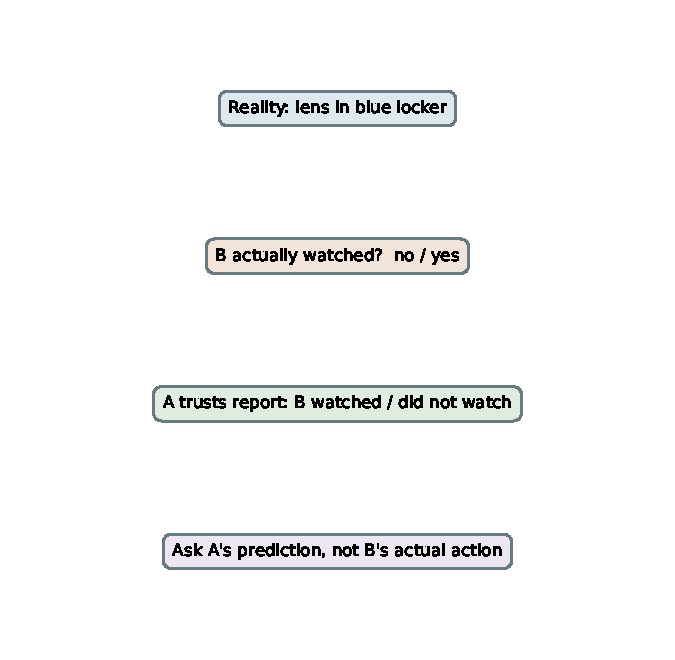
\includegraphics[width=\linewidth]{02/results/belief_intervention.pdf}
\caption{二次信念の対照設計。相手の実際の情報と、予測者が信用する報告を分離する。質問は相手の実行動ではなく予測者による予測を求める。}
\end{figure}

皮肉では、同じ肯定表現に対して仕事の失敗と成功という文脈を変えた。
失言では、作者の目の前で作品を批判した発言者について、作者を知らなかった場合と知っていた場合を区別した。
どちらも相手は傷つきうるので、「失礼かどうか」と「作者を知らないことによる失言かどうか」を同一視しない。
情報不足群では、褒め言葉しか残っていないメッセージから、皮肉か称賛かを確定できるかを問う。

\subsection{回答取得と採点}
作成後のv2プロンプトJSONを固定し、親会話を引き継がない二つの新規コンテキストのCodexサブエージェントへ渡した。
各回答者が読めるファイルを上記の刺激JSON一つに限定し、正解・群分け・生成コード・旧版データ・相互の回答を見せず、選択肢と短い根拠を保存した。
モデルは\texttt{gpt-6.1-sol}、実施日は2026年11月17日である。
温度など内部の生成設定は取得できない。
各コンテキストには44項目を一括提示しており、項目ごとに独立した44会話を作ったわけではない。
問題と条件には共有構造もあるため、88件を独立した標本として検定しない。
元データ、生回答、正解、採点コード、刺激のSHA-256ハッシュを保存し、取得後に監査できる構成とした。

\subsection{修正版の実測結果と対照}
両コンテキストとも44/44項目を正答し、20/20組の最小対に成功した。
コンテキスト間の選択肢一致も44/44であった。
二次信念で実際の知識と予測者の信念が食い違う8項目も、両コンテキストとも8/8正答した。
常にA、B、Cを選ぶ対照はそれぞれ14/44、14/44、16/44であった。
信念2群で常に物の最終場所を答える対照は12/24、二次信念群で相手の実際の知識だけから答える対照は8/16である。

\begin{table}[tb]\centering\footnotesize
\caption{v2の群別正答数。最小対は両問正答で1組とする。44項目の全文と個別の短い根拠は公開JSONに保存。}
\begin{tabular}{lrrr}\toprule
項目群 & 項目数 & 文脈1 & 文脈2\\\midrule
一次信念 & 8 & 8 & 8\\
二次信念 & 16 & 16 & 16\\
皮肉 & 8 & 8 & 8\\
失言の知識 & 8 & 8 & 8\\
情報不足 & 4 & 4 & 4\\
\midrule
最小対の両問正解 & 20組 & 20 & 20\\
\bottomrule\end{tabular}

\end{table}

\begin{figure}[tb]\centering
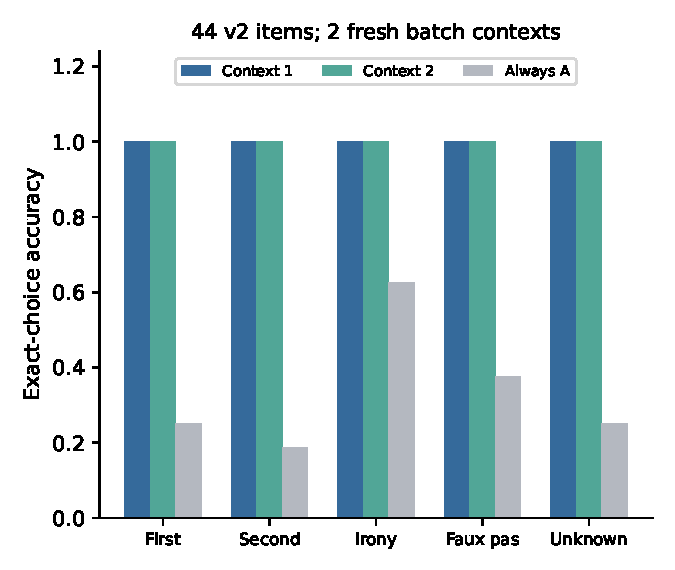
\includegraphics[width=\linewidth]{02/results/accuracy.pdf}
\caption{二つの新規コンテキストと固定回答対照の正答率。二次信念は16項目、一次・皮肉・失言は各8項目、情報不足は4項目。}
\end{figure}

例えば、実際には航が映像を見ていないが綾が見たと信じる項目で、文脈1は「綾は航が映像を見たという報告を信じているため、実際の故障にかかわらず青いロッカーを探すと予測する。」と説明した。
反対方向の不一致にも対応し、岳が澪は見ていないと信じる場合は、澪が実際に見ていても元の棚を選んだ。
情報不足群では、両コンテキストとも称賛か皮肉かを無理に確定しなかった。
これらは、今回の明示的で短い日本語物語では、現実・相手の情報・予測者の信念を区別した答えを生成できたという観察である。
一方、全問正解という天井効果のため、能力の上限や誤りやすい境界は特定できなかった。
信頼する報告の文言を対応づける規則でも解ける構成なので、柔軟なToMの獲得まで結論を広げない。

\subsection{ヒトとの類似性・相違と今後のデータ}
ヒトとの類似性は、観察していない出来事を他者が知らないと扱い、同じ言葉を状況に応じて解釈し、情報不足を認めるという出力の特徴にある。
一方、人間は視線・声の調子・身体の動き・過去の対人関係からも判断する。
今回のLLMは、情報アクセスや報告への信用を実験者が明示した文章から解いた。
人間の対照群を測定していないため、100\%という結果から人間以上と結論づけることはできない。
出題にも同系列のLLMを利用しており、出題側と回答側の独立性にも限界がある。
また、識別子と表示順の監査で既知の抜け道は除いたが、あらゆる表面的な解法を排除できたとは主張しない。

類推推論では、レンズ・センサー・鍵・基板といった対象の置換だけでなく、「他者が接した情報によって信念を更新する」という関係を別の課題に対応させられるかが焦点になる。
例えばソフトウェアのアクセス権、共同作業の共有履歴、誤った地図を使う相手との協調へ移すテストが考えられる。
この種の類推は強いAIの研究に有用な仮説だが、その十分条件が証明されたわけではない。

今後集めるべきデータは、各人物が各時点で何を見聞きしたかを注釈した時系列対話、情報を隠す協調課題、誤解を指摘した後に信念を修正する長期的対話である。
正解ラベルに加えて、情報不足による不確実性、文化や関係性の違いで複数解が妥当になる範囲も記録したい。
評価では作成者とモデル系列を分け、未公開項目を独立に作り、文順・言い換え・不要情報・暗黙の観察機会への頑健性を調べる必要がある。
公開後に同じ項目で将来モデルを測る場合には、学習データへの混入も考慮すべきである\cite{tomreview}。
\repolink{02}
\clearpage
\section{第3問：弁当づくりで理解する進化計算}
\subsection{身近な例と遺伝子の対応}
16区画の弁当に8種類の食材を詰める問題を考える。
各区画の食材番号が遺伝子であり、16個を並べたものが染色体となる。
例えば、ご飯・鶏肉・卵・豆腐・ブロッコリー・人参・豆・果物を番号0〜7で表す。
一つの弁当が個体、48個の弁当案が集団である。
どの食材も単独では目的を満たせず、組合せが重要になる。
栄養・予算・種類数の係数は、説明のため著者が定めた架空の値である。
食品成分表からの実測値ではなく、実際の食事を推奨する実験ではない。

集団初期化では、各区画へ独立に食材を無作為配置する。
適合度計算ではカロリー$K$、タンパク質$P$、費用$C$、野菜区画数$V$、食材ごとの区画数$c_j$を計算し、次の罰点$L$を小さくする。
\[
\begin{split}
L={}&\left(\frac{K-520}{45}\right)^2
+\left(\frac{(30-P)_+}{3}\right)^2\\
&+\left(\frac{(C-480)_+}{30}\right)^2+(4-V)_+^2\\
&+0.15\sum_j(c_j-5)_++0.25(8-D).
\end{split}
\]
ここで$(x)_+=\max(0,x)$、$D$は含まれる食材の種類数である。
栄養への近さに加え、予算超過・野菜不足・同一食材の過多・種類の少なさを評価する。
進化計算は人間の価値判断を自動的に作るわけではない。
何を「良い弁当」と定義したかが、そのまま結果に反映される。

\begin{figure}[tb]
\centering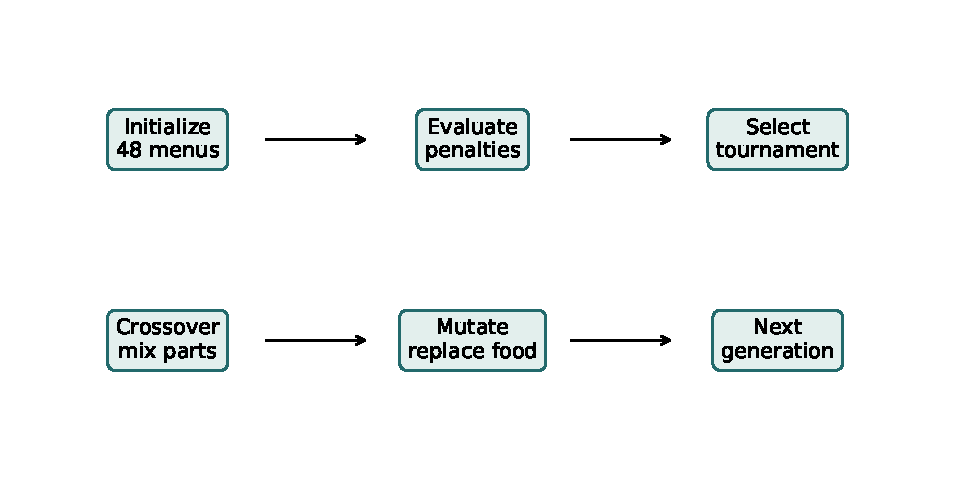
\includegraphics[width=\linewidth]{03/results/evolution_cycle.pdf}
\caption{弁当案の世代交代。選択・交叉・突然変異・評価を反復する。図は実装に対応した自作図。}
\end{figure}

選択・淘汰では、無作為に3案を選び、罰点が最も小さい案を親にするトーナメント選択を行う。
交叉では、親Aの前半と親Bの後半をつなぐ。
「ご飯と主菜の組合せ」と「副菜の組合せ」を異なる親から受け継ぐイメージである。
16区画の表現なので、交叉後も区画数は必ず16に保たれる。
突然変異では各区画を確率$1/16$で8種類から再抽選する。同じ食材も含むため、実際に食材が変わる確率は$7/128$である。この操作により親にない組合せを導入できる。
世代交代では48個の子を次世代とし、これまでの最良案を1個保存するエリート保存を加える。
最良案の罰点は悪化しないが、集団の多様性が維持される保証はない。

\subsection{コードで確かめる探索の改善}
人口48、60世代、乱数種0〜9の10試行を用いた。
初期集団を含め、各方式は2,928回の適合度評価を行う。
GAに加えて、交叉と選択だけで突然変異を除いた方式、毎回48案を独立に生成する無作為探索を比較した。
位置を入れ替えただけの弁当は同じ評価になるので、全ての食材個数ベクトル
$\sum_{j=0}^{7}c_j=16$を列挙して、最適値も独立に調べた。
その総数は$\binom{23}{7}=245,157$である。
遺伝子配列には同じ個数を表す重複があることを明記し、GAがこの全列挙より理論的に優れるとは主張しない。

\begin{table}[tb]\centering\small
\caption{10試行の最終罰点と厳密最適値への到達回数。全方式で評価回数は同一。}
\begin{tabular}{lrr}\toprule
方式 & 罰点の中央値 & 最適到達\\\midrule
GA & 0.23901 & 8/10\\
突然変異なし & 0.25494 & 2/10\\
無作為探索 & 0.30883 & 1/10\\\bottomrule
\end{tabular}\end{table}

全列挙による最適罰点は0.2390123457であり、食材個数の一例は
$(4,4,1,1,1,3,1,1)$であった。
表の通りGAの中央値はこの値と一致したが、2試行は最適値に届かなかった。
図の帯は乱数種間の四分位範囲であり、世代ごとの個体のばらつきではない。
突然変異を除くと、初期集団から失われた食材や配列部分を回復しにくくなり、早い段階で改善が止まる例が見られた。
この実験は、一つの評価関数において変異が役立つことを示す。
あらゆる最適化問題でGAが無作為探索に勝つという結論にはならない。

\begin{figure}[tb]\centering
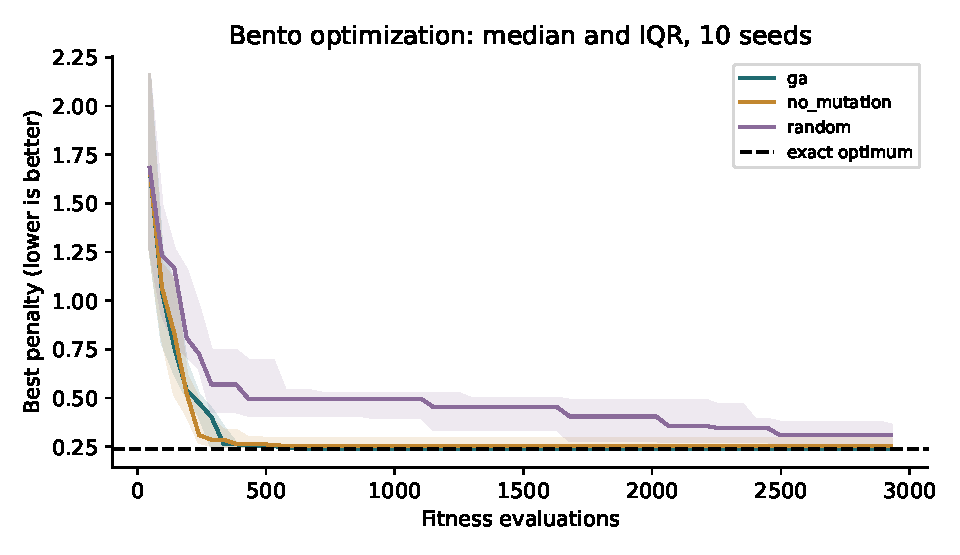
\includegraphics[width=\linewidth]{03/results/convergence.pdf}
\caption{最良罰点の中央値と四分位範囲。横軸を世代数でなく評価回数にそろえた。}
\end{figure}
\begin{figure}[tb]\centering
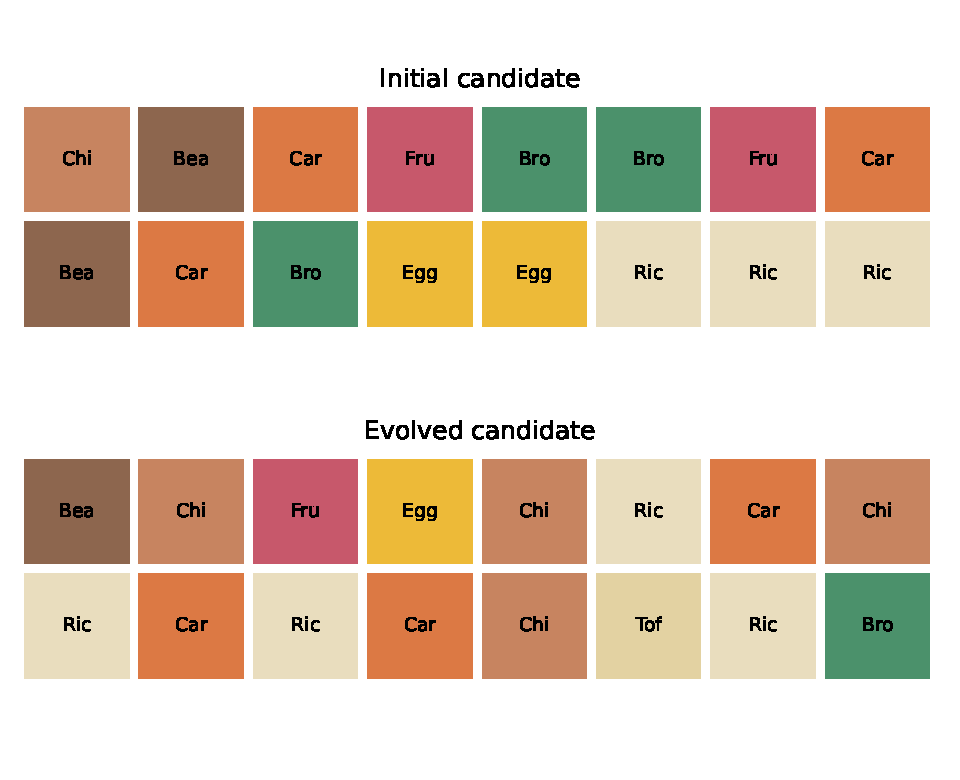
\includegraphics[width=\linewidth]{03/results/bento.pdf}
\caption{初期案と進化後の案。色は食材を表す。見た目の配置自体は今回の適合度に含めていない。}
\end{figure}

\subsection{応用例：細胞を集めるXenobotの形状設計}
課題の除外一覧にない応用として、Xenobotの形状設計を取り上げる。
これは既に工場で使われる製品というより、進化計算が実物の生物工学実験に接続した研究応用である。
研究者はカエル由来の細胞からなる小さな集合体を用い、周囲のばらばらの細胞を集める能力を調べた\cite{xenobot}。
進化的探索は、コンピュータ内で形状候補を評価し、細胞を集めやすい形を探すために使われた。
口の開いた形状を持つ集合体が、動きながら細胞をまとめるという機構は、「皿の上の細かい粒を、へらの形を変えて集める」と考えると理解しやすい。

\begin{figure}[tb]\centering
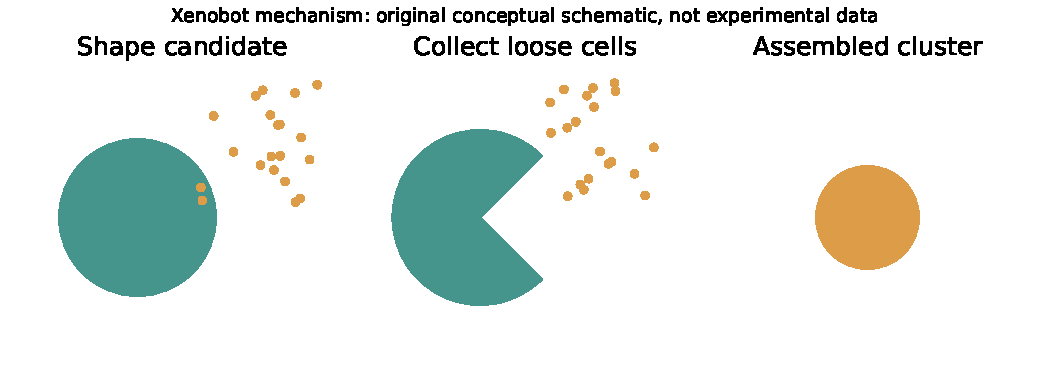
\includegraphics[width=\linewidth]{03/results/xenobot_schematic.pdf}
\caption{形状と細胞収集の関係を説明する独自の概念図。論文の顕微鏡画像や、本レポートによる生物実験の結果ではない。}
\end{figure}

弁当の例と対応させると、遺伝子は食材番号から形状のパラメータへ、適合度は栄養と予算から細胞を集めて次の集合体を生む能力へ置き換わる。
ここで「進化する」のは計算機内の設計候補であり、生物のDNAをGAが直接書き換えるという意味ではない。
研究チームの解説でもシミュレーションによる形状探索と実物の組立てが説明されている\cite{wyss}。
計算機の予測が実物でも成り立つかを調べる点が、この応用の重要な部分である。

この例が面白い理由は、制御プログラムだけでなく、\emph{形そのものが仕事をしやすくする}点にある。
弁当の最適値が評価式に依存したように、Xenobotでもシミュレータ、環境、測定する仕事を変えれば有利な形は変わりうる。
細胞の集まり方を正しくモデル化できなければ、計算上の高得点が実物の成功につながらない。
本レポートの弁当デモは進化計算の原理を説明するもので、Xenobotの物理や生物実験を再現したものではない。
\repolink{03}
\clearpage
\section{第4問：小町算の探索と高精度な$\sqrt{2}$近似}
\label{sec:q04}

\subsection{探索目標と有限な文法}
数字$1,2,\ldots,9$を各1回、順番通りに用いる条件で、式$e$の値$v(e)$を$\sqrt{2}$へ近づけた。
探索法そのものの比較と、精度を追求する追加探索を実施した。
課題ページの$\sqrt{2}$の表示には誤植があるため、正しい値
$1.414213562373095\ldots$を基準にする。
元の式を有理数で再計算すると、順序固定の例は$6883/4867$で、絶対誤差は$4.6418595\times10^{-6}$である。
並べ替え例のうち最初の式も、実際には$390050/275807=1.41421356238239\ldots$となる。
元の数式と表示された近似小数を区別して検証した。

式の文法を明示しないと、階乗の繰り返しなどで探索空間が際限なく増える。
本実験では、葉を「連続する数字の連結整数」「その連結に小数点を1個入れた値」「1桁の数字の階乗」のいずれかとし、内部節点を四則演算とした。
複合式全体の階乗は含めない。
ゼロ除算を除外し、途中値の絶対値を$10^9$以下、既約分母を80 bit以下に制限した。
以下の完全性・最短性は、この有限な文法内での性質である。
小数は例えば$.12=3/25$として扱い、状態のキーには浮動小数点数を使わない。

\subsection{同じ状態グラフでDFS・BFS・A*を比較する}
逆ポーランド記法の状態を
\[
 s=(i;v_1,\ldots,v_k)
\]
と定義した。$i$は使用済み数字数、後半は有理数のスタックである。
未使用の連続数字から葉を1個積む操作と、上位2値を四則演算で1値にまとめる操作を生成する。
全数字を消費してスタックが1個となり、
$|v_1-\sqrt{2}|\leq\varepsilon$を満たせば目標である。
同一の$(i;v_1,\ldots,v_k)$は統合し、代表となる数式文字列を保存した。
後継生成順序、値の範囲、目標判定、重複判定、展開予算は全方式で共通である。

経路コスト$g(s)$は、葉の追加と二項演算を各1とした操作数である。
残り数字があれば、それを全部連結した1個の葉を追加できると緩和し、次の下界を設計した。
\[
 h(s)=\begin{cases}
 k+1,&i<n,\\
 \max(0,k-1),&i=n.
 \end{cases}
\]
前者では追加が少なくとも1回、その後の統合が少なくとも$k$回必要となる。
後者では$k$値の統合に最低$k-1$回かかる。
いずれの遷移でも$h(s)\leq1+h(s')$が成り立つため、許容的かつ整合的な下界となる。
A*は$f=g+h$の小さい状態から取り出し、より小さい$g$で到達した状態を更新する。
これはA*の最小コスト探索の原理\cite{hart1968}に対応する。

さらに同じ$f$の状態について、現スタック上端と残余数字から作れる葉を1回だけ演算したときの$\sqrt{2}$への近さで整列した方式をA*+とした。
近さを表す値そのものには許容性を主張せず、\emph{同一$f$内の優先順位}だけに用いた。
このため、目標発見時の最小操作数の保証を保ちながら、巨大な同点集合の探索順を改善できる。
評価にはヒューリスティックの計算時間も含めた。

\begin{table}[tb]
\centering\small
\caption{目標までの展開状態数。A*+は近さによる同点整列を加えたA*。$\dagger$は予算到達による打切り。}
\label{tab:q04nodes}
\begin{tabular}{lrrrr}
\hline
数字数$n$ & DFS & BFS & A* & A*+\\
\hline
3 & 22 & 98 & 69 & 7\\
4 & 2,266 & 4,881 & 5,362 & 1,683\\
5 & 39,162 & 70,851 & 65,263 & 30,855\\
9 & 16,258 & $100,000^{\dagger}$ & 30,360 & 990\\
\hline
\end{tabular}
\end{table}

実験は$n=3,4,5,9$に対し、それぞれ$\varepsilon=10^{-1},10^{-2},10^{-3},10^{-3}$、最大10万展開とした。
小規模問題は比較機構を確認するための例題であり、$n$と同時に許容誤差も変えているため、行間の比を計算量の増加率とは解釈しない。
展開数は後継を実際に生成した非重複状態数であり、目標として取り出した節点は含めない。
生成数・訪問状態数・フロンティアの最大登録数も別途JSON/CSVに保存した。

\begin{figure*}[tb]
\centering
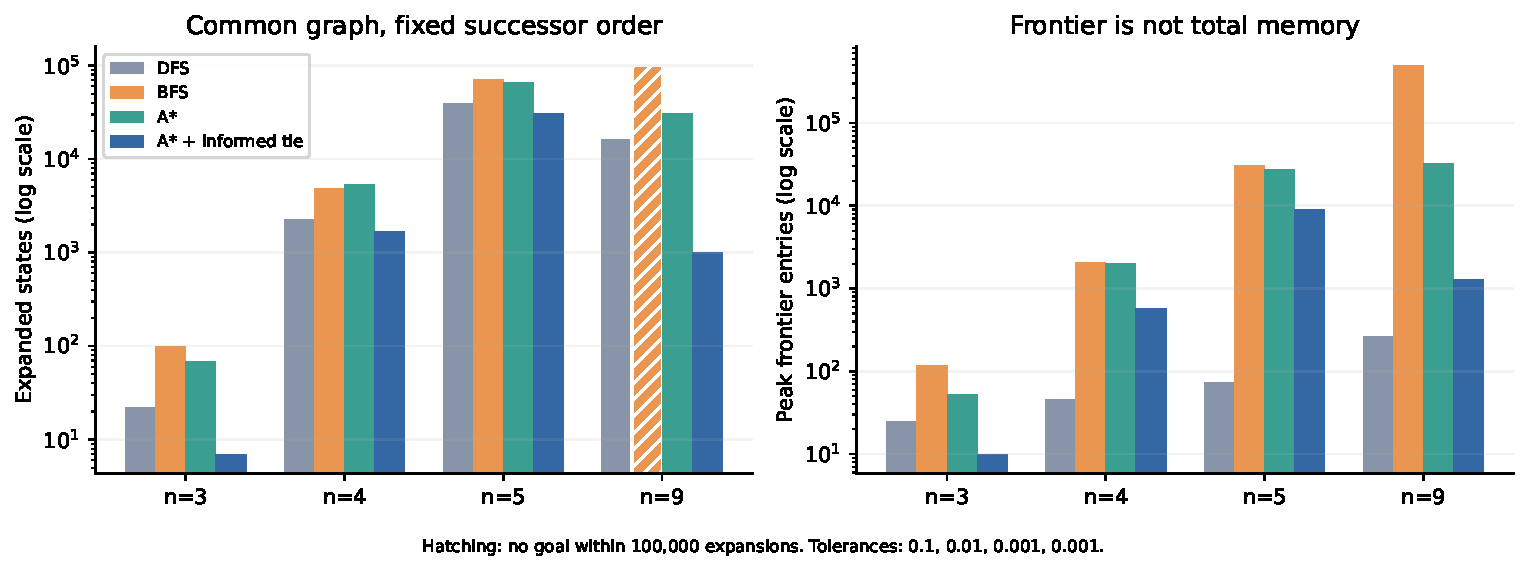
\includegraphics[width=.96\textwidth]{04/results/search_comparison.pdf}
\caption{共通状態グラフに対する探索の実測。左は展開数、右はフロンティア最大登録数。斜線は予算10万展開での打切りであり、解の不存在を意味しない。DFSも重複判定用辞書を保持するため、フロンティアが小さくても総メモリが定数になるわけではない。}
\label{fig:q04search}
\end{figure*}

表\ref{tab:q04nodes}と図\ref{fig:q04search}より、素朴なA*が常にDFSやBFSより少ない展開数になるわけではない。
$n=4$ではA*の5,362展開に対し、BFSは4,881展開であった。
下界が正しくても弱い場合、同点の並びが結果に影響するためである。
一方、A*+では全4例で展開数が減少した。
特に9桁ではA*の30,360から990へ減り、約30.7倍の差となった。
ただし決定論的な4例の結果であり、一般の数列や任意の目標値に対する優越性は主張しない。

9桁の場合、DFSは17操作で$99/70$を発見し、A*とA*+は5操作で
\[
 \frac{1.234}{.56}-.789
 =\frac{4951}{3500}
\]
を得た。
後者の絶対誤差は$3.5786620\times10^{-4}$、前者は$7.2151913\times10^{-5}$である。
すなわち、最短の式と最も正確な式は一致しない。
9桁の実測時間はDFSが0.123秒、BFSが打切りまで5.773秒、A*が0.437秒、A*+が0.061秒であった。
時間はmacOS 15.5/arm64、Python 3.9.6での1回の観測値であり、反復測定した平均ではない。
BFSの最大フロンティアは495,949登録に達した。

\subsection{区間DPと逆算による高精度探索}
高精度を要求すると通常の列挙探索は膨大になる。
そこで数字列を$1234\mid56789$または$12345\mid6789$に分け、左右それぞれの全ての括弧付けを区間動的計画法で列挙した。
各区間の辞書は「有理数$\mapsto$最小の演算子数を持つ代表式」とする。
左右の値の全組合せを根で試す代わりに、目標から逆算した右側の値を二分探索する。
例えば根が除算なら$a/b\simeq\sqrt{2}$に対し$b\simeq a/\sqrt{2}$を探す。
他の三則も同様に扱い、近傍候補と端点を検証した。
最終結果の誤差はDecimal 60桁で再計算した。
二分探索の位置決定には倍精度数を用いるため、これは測定した候補からの高精度解であり、全構文の大域最適性を主張するものではない。

\begin{figure}[tb]
\centering
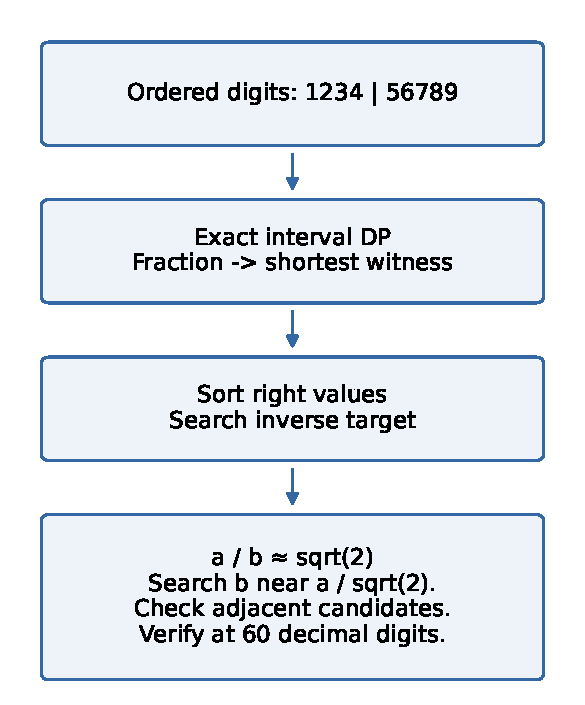
\includegraphics[width=\linewidth]{04/results/mitm_pipeline.pdf}
\caption{部分式を有理数の辞書に圧縮し、根の演算を逆算して組み合わせる。DFS/BFS/A*の実験にはこの前計算を使用していない。}
\label{fig:q04pipeline}
\end{figure}

$4\mid5$分割では、左に2,975、右に265,046種類の有理数が存在した。
根で単純に全組合せを作れば、四則それぞれについて約$7.9\times10^8$組を調べる必要がある。
逆算による候補照合は83,293回で済み、前計算込みの実測は約4秒であった。
順序固定で得られた式は
\begin{equation}
 \frac{(.1+2/.3)-.4}
 {\left(.5+\dfrac{6/.7}{8!}\right)9}
 =\frac{149744}{105885}.
 \label{eq:q04ordered}
\end{equation}
この値は$1.4142135335505501\ldots$、絶対誤差は
$2.8822545\times10^{-8}$である。
課題ページの順序固定例より約161倍小さい誤差となった。
各数字の使用順序は$1,2,3,4,5,6,7,8,9$であり、追加の数字定数を使用していない。

\subsection{数字を並べ替えた場合と「美しさ」}
固定した3つの並べ替え$987654321$、$371526498$、$824613975$について、同じ$4\mid5$分割を試した。
このうち$371526498$から
\begin{equation}
 \frac{3\{(.7+1)-5\}}
 {2-\dfrac{.6\times4!+9!}{8!}}
 \label{eq:q04permuted}
\end{equation}
を得た。絶対誤差は$1.8404692\times10^{-9}$であり、式\eqref{eq:q04ordered}より約15.7倍小さい。
ただし順列$9!$通りの網羅探索ではない。
並べ替えによって表現可能な分数が増え、良い近似に出会う機会は増すが、試したどの順列でも改善するわけではなかった。
課題ページの並べ替え例の誤差$9.2955\times10^{-12}$は、今回得た最良値よりさらに小さい。
したがって、今回の探索は既知例を上回る最高精度の達成を示すものではない。

\begin{figure*}[tb]
\centering
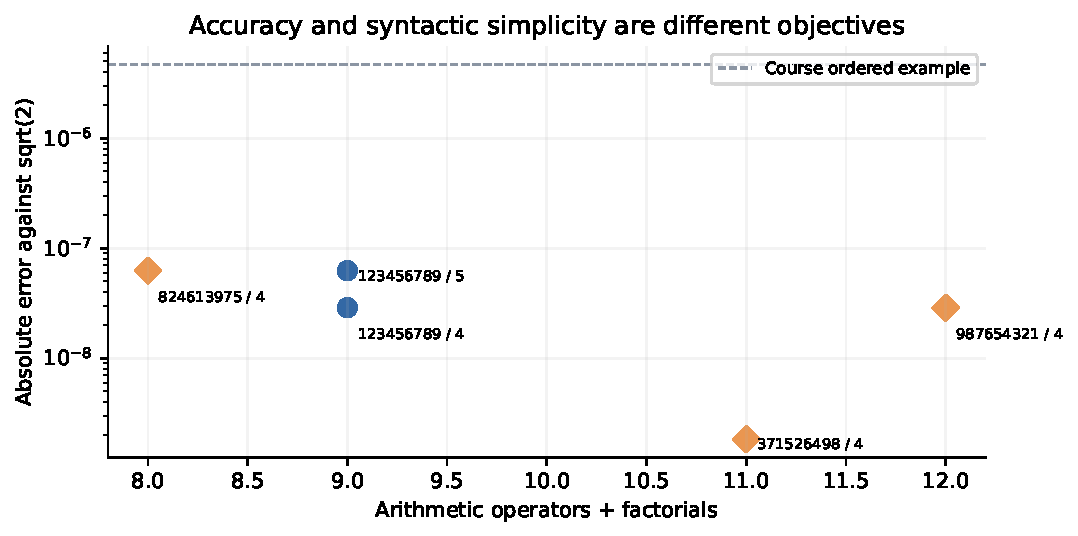
\includegraphics[width=.85\textwidth]{04/results/precision.pdf}
\caption{独立した高精度探索で得た式の精度と演算子数。丸は順序固定、菱形は並べ替え。図中の末尾の4または5は分割位置。階乗も演算子1個として数える。}
\label{fig:q04precision}
\end{figure*}

式の美しさは、精度とは別に、二項演算と階乗の合計個数、次いで括弧を含む文字数で評価した。
辞書内で同値の式を統合する際には、この順に短い表現を残した。
しかし最終候補はまず絶対誤差を優先して選んだため、図\ref{fig:q04precision}の各点は多目的最適化の完全なPareto前線ではない。
例えば、A*が得た2個の二項演算だけの式は読みやすい一方、式\eqref{eq:q04ordered}は9演算子、式\eqref{eq:q04permuted}は11演算子を要する。
用途に応じて許容誤差を先に決め、その範囲で最短の式を選ぶ方法が、近似と簡潔さを両立させやすい。

\subsection{実装上の工夫と残る課題}
実装では式と値を保持する不変データ型、四則演算、後継生成、探索方策、実験・描画を分離した。
数式文字列を実行する\texttt{eval}は使用しない。
単体テストでは小数・階乗の厳密値、ゼロ除算の排除、下界の整合性、小規模なRPN列挙と区間DPの到達値集合の一致、A*とBFSの最小操作数の一致を確認した。
元ページの近似値の誤植も有理数と60桁小数の両方で確認し、全パラメータと生結果を公開対象にした。

今後は全ての根の分割位置を扱う区間DP、式木の高さを加えた美しさの評価、より厳しい精度での探索法比較が考えられる。
現実装の下界は「あと何手か」という構造だけを見るため、値の到達可能性を表す区間や合同条件を許容的に組み込めれば、同点整列だけに依存しない削減が期待できる。
また、元の課題にある8パズルと異なり、全ての解の深さが同じとは限らないことを、連結を含む今回の文法で実際に確認できた。

\repolink{04}
\clearpage
\section{第5問：3次元HPモデルと学習形質の遺伝}
\label{sec:hp}

\subsection{問題設定と比較の考え方}
HPモデルはアミノ酸を疎水性Hと極性Pの2種類に簡略化し、鎖を格子上に置くモデルである。本実験では立方格子を用い、同じ格子点に2残基を置かず、鎖の隣接残基間のマンハッタン距離を1とする。鎖に沿って隣り合わないH同士が格子上で接したときにエネルギーを1下げる。
\begin{equation}
 E(r)=-C_{HH}(r).
\end{equation}
ここで$C_{HH}$は、$j>i+1$、$s_i=s_j=H$、$\|r_i-r_j\|_1=1$をすべて満たす残基対$(i,j)$の数である。したがって小さい$E$ほどよい。P間接触とH--P接触には得点を与えない。

集団内の構造を交叉と突然変異で改善する考え方はUngerとMoultの先行研究を参考にした\footnote{R. Unger and J. Moult, ``Genetic Algorithms for Protein Folding Simulations,'' \emph{J. Mol. Biol.}, 231(1), 75--81, 1993. \url{https://doi.org/10.1006/jmbi.1993.1258}}。実装は独自に作成し、同一の実行可能解空間と遺伝演算に対して、学習結果を評価と遺伝のどちらに使うかだけを変更した。実タンパク質の立体構造や折り畳み時間を予測するモデルではなく、探索と学習の相互作用を調べる計算実験である。

\subsection{遺伝子型・表現型と実行可能性}
遺伝子型は原点を始点とする3次元整数座標列である。これは6方向の結合ベクトル列と相互変換できる。重なった構造を罰点で扱う方式では、重なりの解消とH核の形成という異なる課題が適合度に混ざる。そのため、初期化・交叉・突然変異のすべてで自己回避歩行を保持した。

初期集団は空いている隣接格子点から逐次ランダムに成長させ、成長が行き詰まった場合だけ作り直した。交叉は親Aの前半と親Bの後半を、接続点を共有するよう平行移動・回転してつなぐ。回転は立方体の24通りの正規回転から選ぶ。最大8回試して重なりのない子を得られなければ親Aを返す。突然変異は、鎖の後半を回転するpivot変異を確率0.65、末端側の最大12残基を再成長する変異を確率0.35で選ぶ。pivotは最大12回、再成長は最大6回試し、成功しなければ元の構造を残す。失敗も実行時間には含まれる。

学習操作$L(x)$は、末端残基の移動、正方形の対角側へのcorner flip、連続2残基のcrankshaft移動をすべて調べ、エネルギーの減少が最大の移動を採用する最急降下法である。改善がなくなるまで繰り返し、反復回数の打切りは設けない。整数エネルギーが厳密に減少し、下限を持つので必ず終了する。ここで得る局所最適性は、この明示した小近傍に関するものである。等エネルギーの平坦部の横断や大きなpivot操作は含まない。

1回の近傍移動で変わる残基は1個か2個なので、接触エネルギーは変更残基に接する対だけから差分計算した。全再計算との一致、結合長、自己回避性、局所探索終了時の全近傍に対する非改善性を自動テストで確認した。

\subsection{3種類のGAを混同しない実装}
ダーウィン型は遺伝子型$x$の$E(x)$を評価し、そのまま子の生成に使う。ボールドウィン型は$E(L(x))$を評価に使うが、交叉・変異の入力は学習前の$x$である。ラマルク型は$L(x)$自体を遺伝子型に書き戻す。これらを表\ref{tab:hp-inheritance}に示す。選択はエネルギーの小さい個体を優遇する。

\begin{table}[htbp]
\centering
\small
\caption{適合度と継承対象を分けた実装。}
\label{tab:hp-inheritance}
\begin{tabular}{lll}
\hline
型 & 評価する値 & 子に使う構造\\
\hline
Darwin & $E(x)$ & $x$\\
Baldwin & $E(L(x))$ & $x$\\
Lamarck & $E(L(x))$ & $L(x)$\\
\hline
\end{tabular}
\end{table}

特に、ボールドウィン型でエリートとして保存する遺伝子型も$x$のままにした。改善後の構造だけを保存すると、意図せずラマルク型になってしまう。集団の学習前エネルギーと学習後適合度を別々に記録し、両者の違いを検査可能にした。一方、報告用の最良解アーカイブには、局所探索中を含め、実際に評価したすべての構造を記録した。このアーカイブは親選択や集団への再投入には用いない。

\subsection{配列の検査と実験条件}
課題ページの圧縮表記を展開するパーサを作り、掲載された10配列を機械的に検査した。その結果、\textbf{「配列48」とされた第1・第10配列は、掲載文字列をそのまま展開すると47残基だった}。第2--第9配列は48残基である。欠落文字を推測して補うと問題を変更するため、原文と警告を保存し、48残基の比較には第2・第3・第4配列を用いた。課題ページに記載された参照エネルギーは、それぞれ$-34,-34,-33$である。以下ではこれらをs48\_02、s48\_03、s48\_04と呼ぶ。

簡単な対照例として、独自配列toy10=$H^2P^2H^2P^2H^2$、toy20=$(H^2P^2)^4H^4$を加えた。toy10は最初の結合を$+x$方向に固定して、自己回避歩行を全列挙した。この固定は剛体回転による対称性の除去であり、最適値を変えない。完全な歩行308,981本、途中の歩行を含む390,769ノードを調べ、\textbf{最適値$E=-4$を厳密に確認した}。toy20と48残基配列には全列挙による最適性の保証はない。

各配列・各手法についてseed 0--4の5試行を行い、計75試行とした。各seedの初期集団は3手法で同一にし、初期化とその後の遺伝操作には別の乱数系列を使った。集団サイズ32、トーナメントサイズ3、エリート2、交叉確率0.8、変異確率0.9、ランダム移入確率0.03は共通である。エリートは再評価しない。

比較の基準は、(a)局所探索の候補評価も含めた30,000構造の評価、(b)60世代、(c)実測時間、の3通りとした。評価回数が30,000に達した瞬間に、実際にその時点までに観測した最良解を保存する。局所探索の途中で閾値に達した場合でも、後から得た改善解は(a)に含めない。その後の局所探索は完了させ、別の条件である(b)を取得するまで走らせる。反対にダーウィン型は60世代での結果を保存後、30,000評価まで続ける。この設計により、評価予算の超過と局所最適性の取り違えを防いだ。

実行環境はmacOS 15.5、arm64、Python 3.9.6であり、75試行全体で9,939,381回の構造評価を行った。各試行を逐次実行し、共通の初期構造生成を前処理として除外し、初期集団の評価から計時した。その後の選択、遺伝操作、局所探索と記録処理を時間に含む。同じホストでは他課題の処理が動く場合があるため、時間はこの実装と環境での観測値として解釈する。

\subsection{解の品質と探索効率}
表\ref{tab:hp-main}は5試行の平均を示す。toy10は全手法・全seedで厳密最適値$-4$に到達した。一方、48残基配列では、どの資源を揃えるかによって順位が変化した。

\begin{table}[htbp]
\centering
\caption{最良エネルギーの平均。同評価数は30,000構造、同世代数は60世代、秒は60世代までの平均経過時間。小さいエネルギーがよい。}
\label{tab:hp-main}
\small
\begin{tabular}{llrrr}
\hline
配列 & 手法 & 同評価数 & 同世代数 & 秒\\
\hline
toy10 & Darwin & -4.0 & -4.0 & 0.06\\
toy10 & Baldwin & -4.0 & -4.0 & 0.29\\
toy10 & Lamarck & -4.0 & -4.0 & 0.24\\
toy20 & Darwin & -11.4 & -11.0 & 0.12\\
toy20 & Baldwin & -11.0 & -11.8 & 0.78\\
toy20 & Lamarck & -11.8 & -12.2 & 0.47\\
s48\_02 & Darwin & -25.2 & -19.4 & 0.24\\
s48\_02 & Baldwin & -16.0 & -23.2 & 2.63\\
s48\_02 & Lamarck & -19.2 & -22.8 & 0.97\\
s48\_03 & Darwin & -22.6 & -20.2 & 0.25\\
s48\_03 & Baldwin & -15.8 & -21.8 & 2.20\\
s48\_03 & Lamarck & -20.8 & -24.4 & 0.84\\
s48\_04 & Darwin & -19.6 & -17.4 & 0.26\\
s48\_04 & Baldwin & -15.6 & -22.8 & 2.11\\
s48\_04 & Lamarck & -19.4 & -22.2 & 0.86\\
\hline
\end{tabular}

\end{table}

\begin{figure*}[t]
\centering
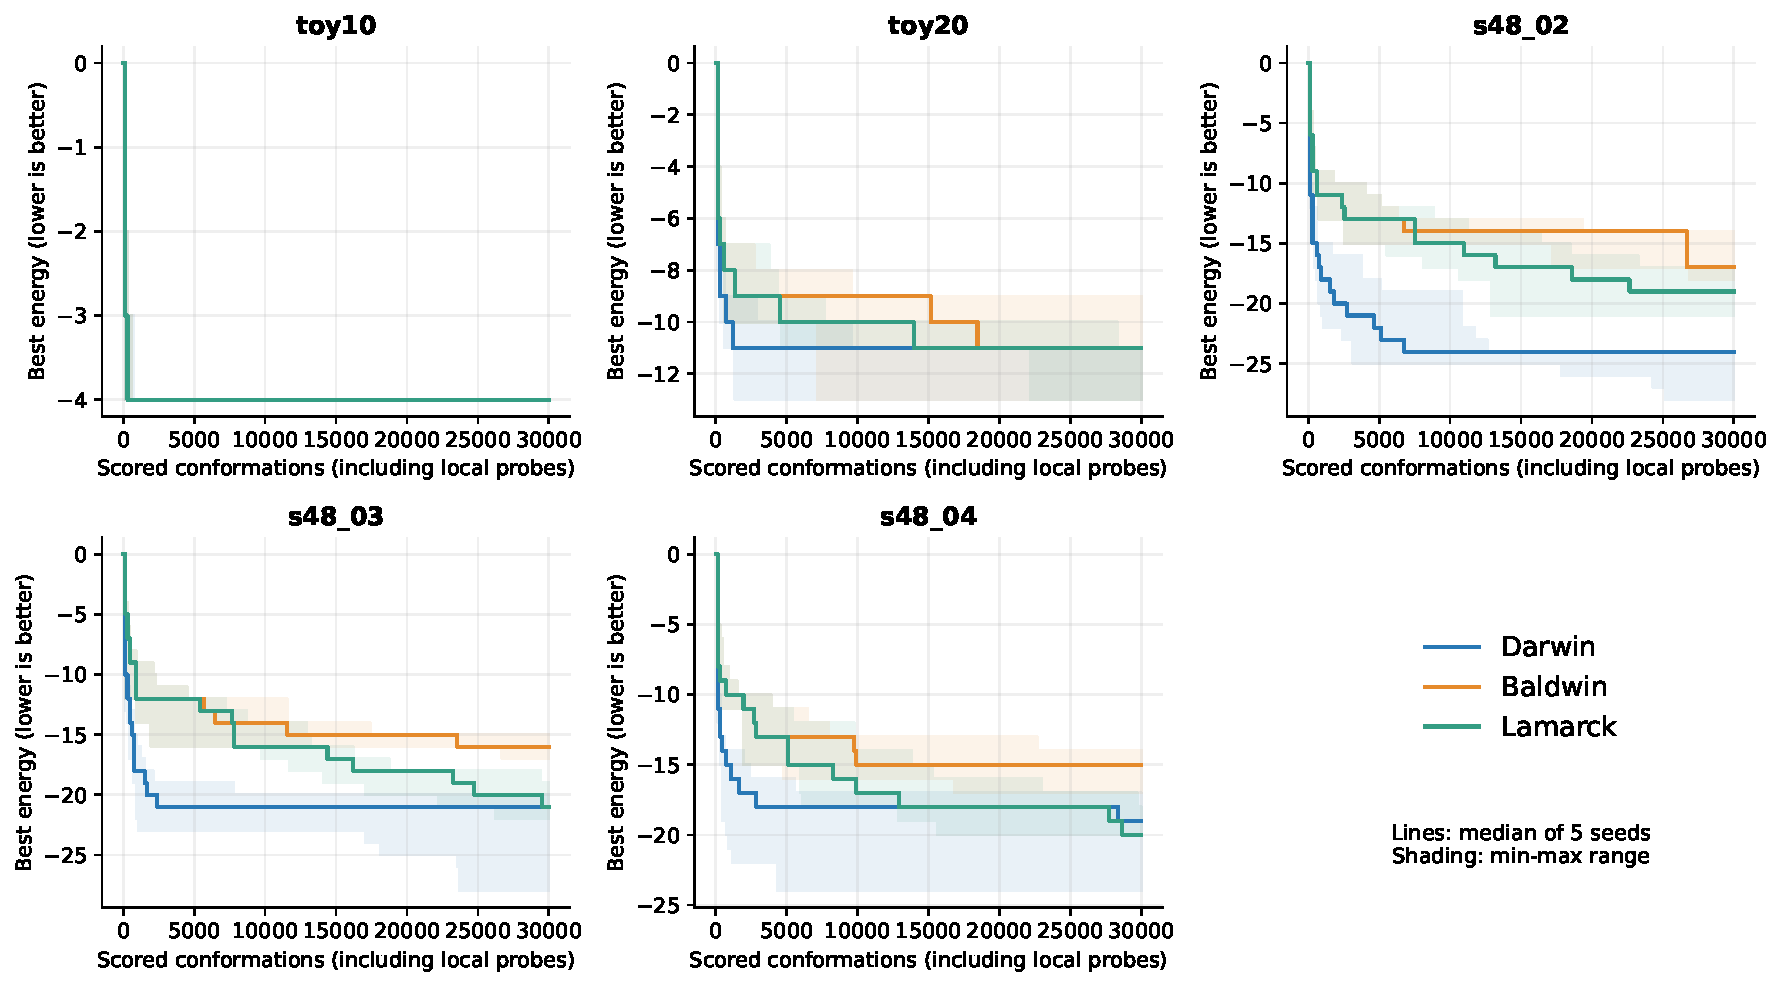
\includegraphics[width=\textwidth]{05/results/convergence_evaluations.pdf}
\caption{評価した構造数を揃えた比較。線は5試行の中央値、陰影は最小値--最大値であり信頼区間ではない。局所探索の近傍候補も1評価として数える。}
\label{fig:hp-eval}
\end{figure*}

\begin{figure*}[t]
\centering
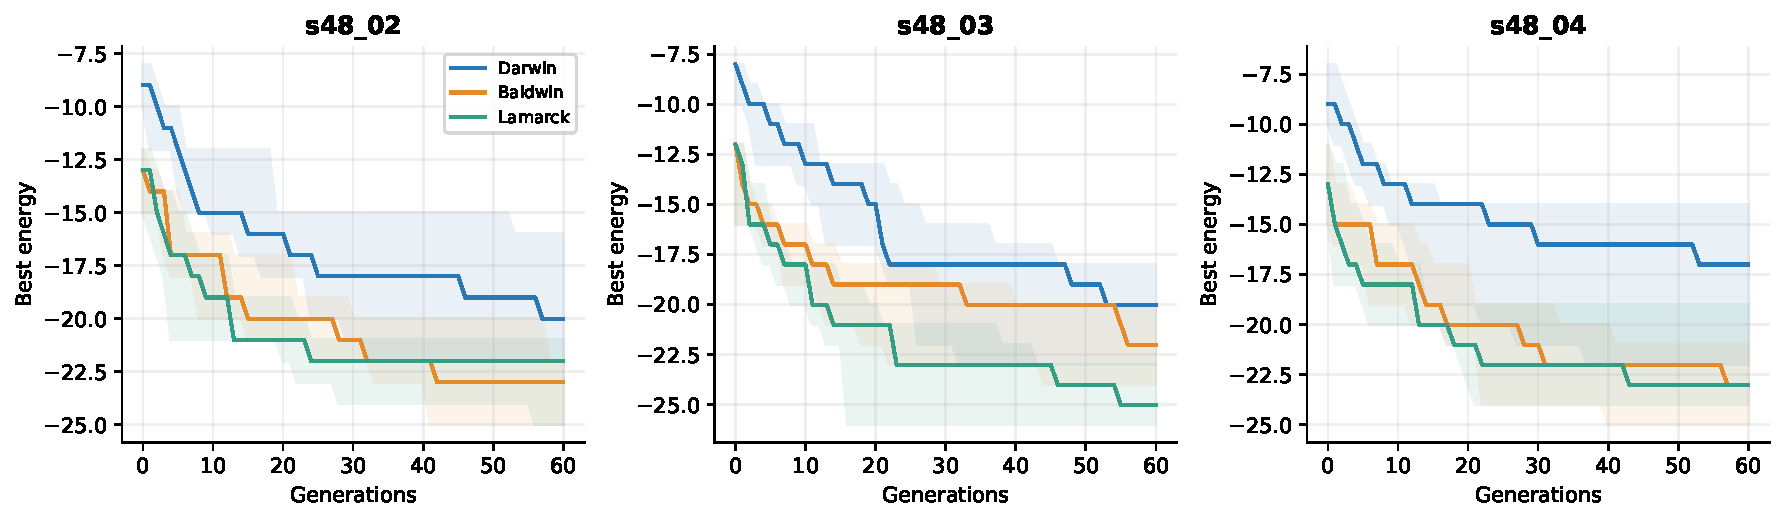
\includegraphics[width=\textwidth]{05/results/convergence_generations.pdf}
\caption{同じ60世代での比較。局所探索による1世代当たりの計算量は共通ではない。}
\label{fig:hp-generation}
\end{figure*}

30,000評価に限ると、s48\_02の平均値はDarwin $-25.2$、Baldwin $-16.0$、Lamarck $-19.2$であり、ダーウィン型が優れていた。試行範囲はそれぞれ$[-28,-24]$、$[-18,-14]$、$[-21,-17]$である。s48\_03でも$-22.6,-15.8,-20.8$と同じ順序であり、s48\_04ではDarwin $-19.6$とLamarck $-19.4$が近かった。局所探索には多くの候補評価が必要なので、少ない評価数を世代更新と大きな構造変化に使う方法が有利になったと解釈できる。

60世代に揃えると、s48\_02は$-19.4,-23.2,-22.8$、s48\_03は$-20.2,-21.8,-24.4$、s48\_04は$-17.4,-22.8,-22.2$となり、学習を行う2手法がいずれもダーウィン型を上回った。例えばs48\_02の60世代までの平均評価数は、Darwin 1,832、Baldwin 449,423、Lamarck 121,913である。ボールドウィン型は改善後の構造を遺伝しないため、各子について再び学習する費用が大きい。したがって、同世代数の優位だけから計算効率の優位を結論することはできない。

\begin{figure*}[t]
\centering
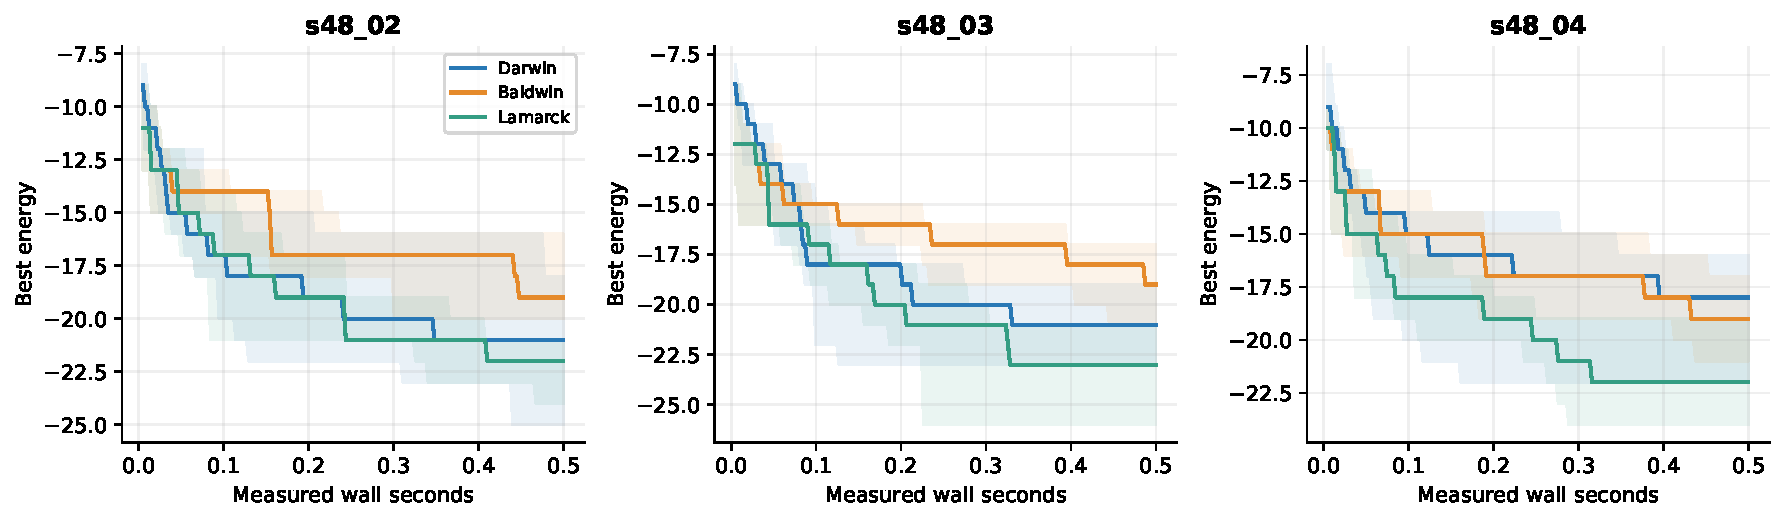
\includegraphics[width=\textwidth]{05/results/convergence_time.pdf}
\caption{48残基の各試行に共通の実測0.5秒までの比較。線は中央値、陰影は試行範囲。局所近傍の差分評価と遺伝操作の費用差が、評価回数基準の順位に影響する。}
\label{fig:hp-time}
\end{figure*}

実時間も揃えると、0.5秒時点の平均値はs48\_02で$-21.6,-18.4,-22.4$、s48\_03で$-20.8,-18.8,-23.2$、s48\_04で$-18.6,-18.8,-22.0$であり、この測定ではラマルク型が3配列とも最もよかった。30,000評価までの平均時間は、例えばs48\_02で4.29秒、0.17秒、0.22秒と大きく異なる。局所探索は変更残基だけを差分評価できる一方、ダーウィン型は1評価ごとに交叉・変異・全接触計算を行うためである。\textbf{「1評価」を同じCPU費用と見なすと、結論を誤る}ことが本実験の主要な知見である。0.5秒比較は保存した改善イベントの時刻から集計したもので、異なる機械でも同じ優劣を保証するものではない。

\subsection{目標水準へ到達するまでの世代と時間}
最良値の比較を補うため、保存済みログに対する補助解析として、s48\_02に共通目標$E\leq-20$を設定した。
これは最適値ではなく、実験後に定めた到達水準である。
60世代以内での初到達を調べ、未達試行は打切りとして残した。
秒は改善イベントの時刻、世代は到達を確認できた最初の世代末の記録を用いる。
\begin{table}[tb]\centering\small
\caption{s48\_02で$E\leq-20$への到達。世代と秒は成功試行のみの中央値であり、全試行の平均ではない。}
\begin{tabular}{lrrr}\hline
手法 & 到達数 & 世代 & 秒\\\hline
Darwin & 3/5 & 51 & 0.205\\
Baldwin & 5/5 & 15 & 0.591\\
Lamarck & 5/5 & 13 & 0.243\\
\hline\end{tabular}

\end{table}
Darwinの成功は3/5、BaldwinとLamarckは5/5であった。
成功した試行ではDarwinの秒の中央値が小さい一方、BaldwinとLamarckは少ない世代でより確実にこの水準へ到達した。
成功試行だけの時間を見れば未達2試行を無視することになるため、到達率との併記が必要である。
目標値や観測期間を変えれば順位も変わりうる。
解析コード\texttt{time\_to\_threshold.py}と各試行の打切り状態も保存した。

\subsection{学習効果と集団の多様性}
学習前の遺伝子型と学習後の表現型を分けて観察すると、手法の違いが明瞭になる。s48\_02、seed 0、60世代のボールドウィン型では、集団の平均遺伝子型エネルギーが$-5.16$、平均学習後適合度が$-14.97$であり、平均9.81接触分の学習改善が残っていた。集団内の最良遺伝子型は$-9$、最良学習後構造は$-23$だった。評価結果が良好でも、その構造自体を継承しているわけではないことが数値から確認できる。

\begin{figure*}[t]
\centering
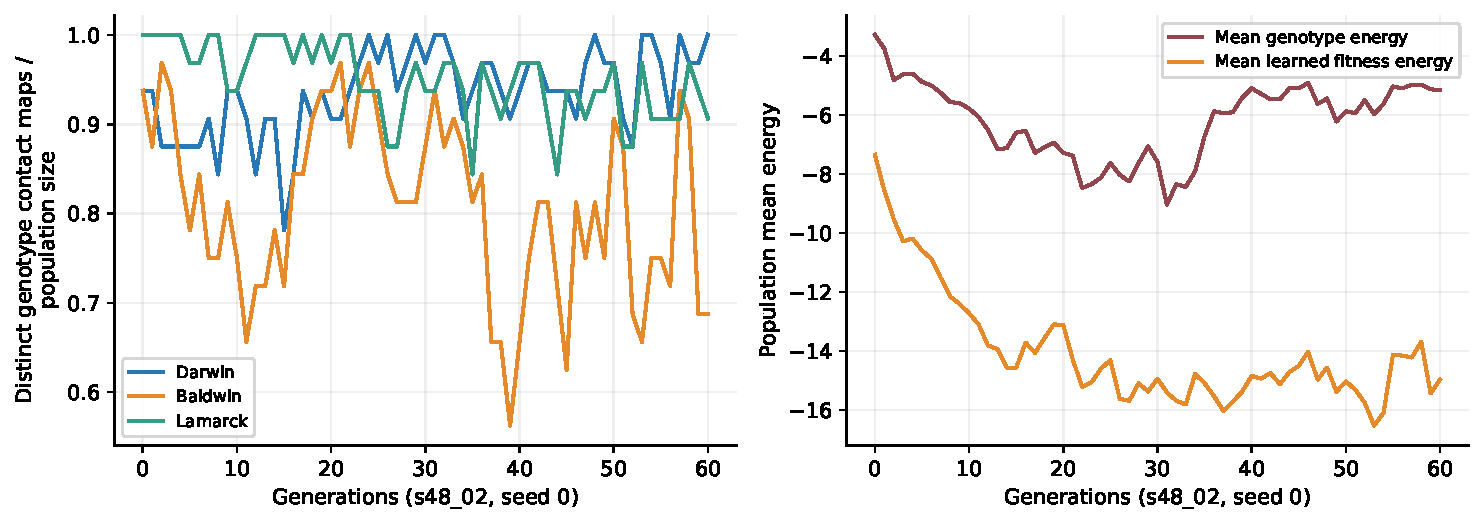
\includegraphics[width=\textwidth]{05/results/learning_and_diversity.pdf}
\caption{s48\_02、seed 0の診断。左は集団内で異なる遺伝子型接触マップの比率、右はBaldwinの学習前後の平均エネルギー。接触マップは回転・平行移動に不変だが、同じ接触集合の異なる構造を区別しない。}
\label{fig:hp-diagnostic}
\end{figure*}

多様性は、集団中の異なるH--H接触集合の個数を集団サイズで割って測った。s48\_02、60世代での5試行平均はDarwin 0.931、Baldwin 0.769、Lamarck 0.925であり、ラマルク型が常に最も多様性を失う、という単純な予想は支持されなかった。接触集合は構造の完全な識別子ではないが、座標の剛体回転だけで見かけ上の多様性が増える問題を避けられる。ここでは移入と大きな変異を併用しており、これらの設定によっても収束の仕方は変わる。

\begin{figure*}[t]
\centering
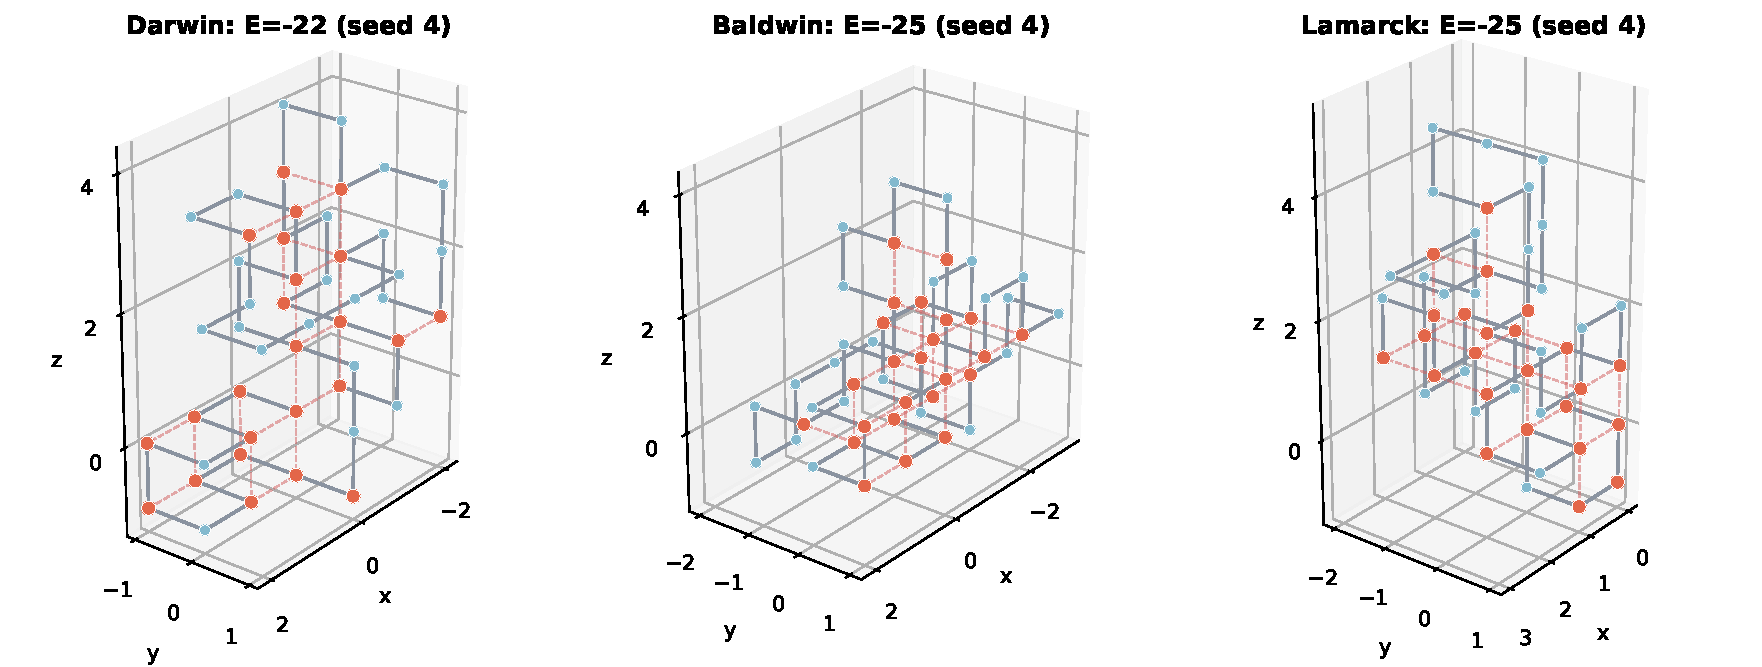
\includegraphics[width=\textwidth]{05/results/folds_3d.pdf}
\caption{s48\_02で60世代時点の最良seedの構造。橙はH、青はP、灰線は鎖、赤の破線は非共有結合H--H接触。Darwin $-22$、Baldwin $-25$、Lamarck $-25$である。異なる評価予算の最良解を混ぜていない。}
\label{fig:hp-folds}
\end{figure*}

\subsection{限界と改善案}
48残基の参照値$-34,-34,-33$は未達成であり、大域最適性は主張できない。小近傍による厳密な局所最適性は、大きな構造移動で改善できないことを意味しない。特にエネルギーが同じ平坦な地形は厳密降下だけでは横断できない。改善案として、非改善移動を一定確率で許す学習、複数の温度を持つ集団、局所学習を適用する個体の割合の適応制御が考えられる。ただし、それらを導入する場合も学習内の費用を計上し、同世代・同評価数・同時間の比較を併記すべきである。

5試行はばらつきを観察するための反復であり、普遍的な優劣や統計的有意差を示すものではない。初期集団は共通だが、学習によって選択された親が変わるため、その後の探索軌道は対応しない。今後はseed数、配列数、交叉不成立率、局所学習費用を増やして評価したい。講義については、学習を適合度だけに反映する場合と遺伝子型に書き戻す場合を、同じ構造の図と費用のグラフで並べると理解が深まると考える。

\subsection{コードと再現手順}
\texttt{hp\_model.py}に構造と遺伝演算、\texttt{experiment.py}に継承規則と計測、\texttt{analyze.py}に図表生成を分離した。\texttt{exact\_toy.py}が小規模厳密解、\texttt{test\_hp\_model.py}が構造・差分・学習規則の検査を担う。配列原文、警告、seed、全改善イベント、各世代の生データと実行環境を保存した。実行コマンドは第5問フォルダのREADMEに示す。

\repolink{05}
\clearpage
\section{第6問：少数三角形による画像近似と美しさの代理目的}
\label{sec:q06}

\subsection{狙いと実験の位置づけ}
画像を多数の画素として記憶する代わりに，少数の三角形の組合せとして表す．本実験では，「三角形を増やして誤差を減らす」だけでなく，輪郭の保持，色のまとまり，ノイズへの頑健性，表現の簡潔さの間にどのような関係があるかを調べた．位置・色・描画順を遺伝子とする間接表現は，Bergらの進化的画像表現とも共通する考え方である\footnote{J. Berg et al., \emph{Evolved Art with Transparent, Overlapping, and Geometric Shapes}, NAIS 2019, \url{https://arxiv.org/abs/1904.06110}．}．実装は独自に作成した．

問題例として，著作権や撮影条件の影響を避けた自作の64\,$\times$\,64 RGB画像3種類を用いた．風景は山・雪・水面などの明瞭な境界，果実は曲線と陰影，勾配画像は連続的な色変化と小さな円形境界を持つ．このように性質を分けることで，単一の絵で得た成功を画像一般の性質と取り違えないようにした．

\begin{figure*}[t]
\centering
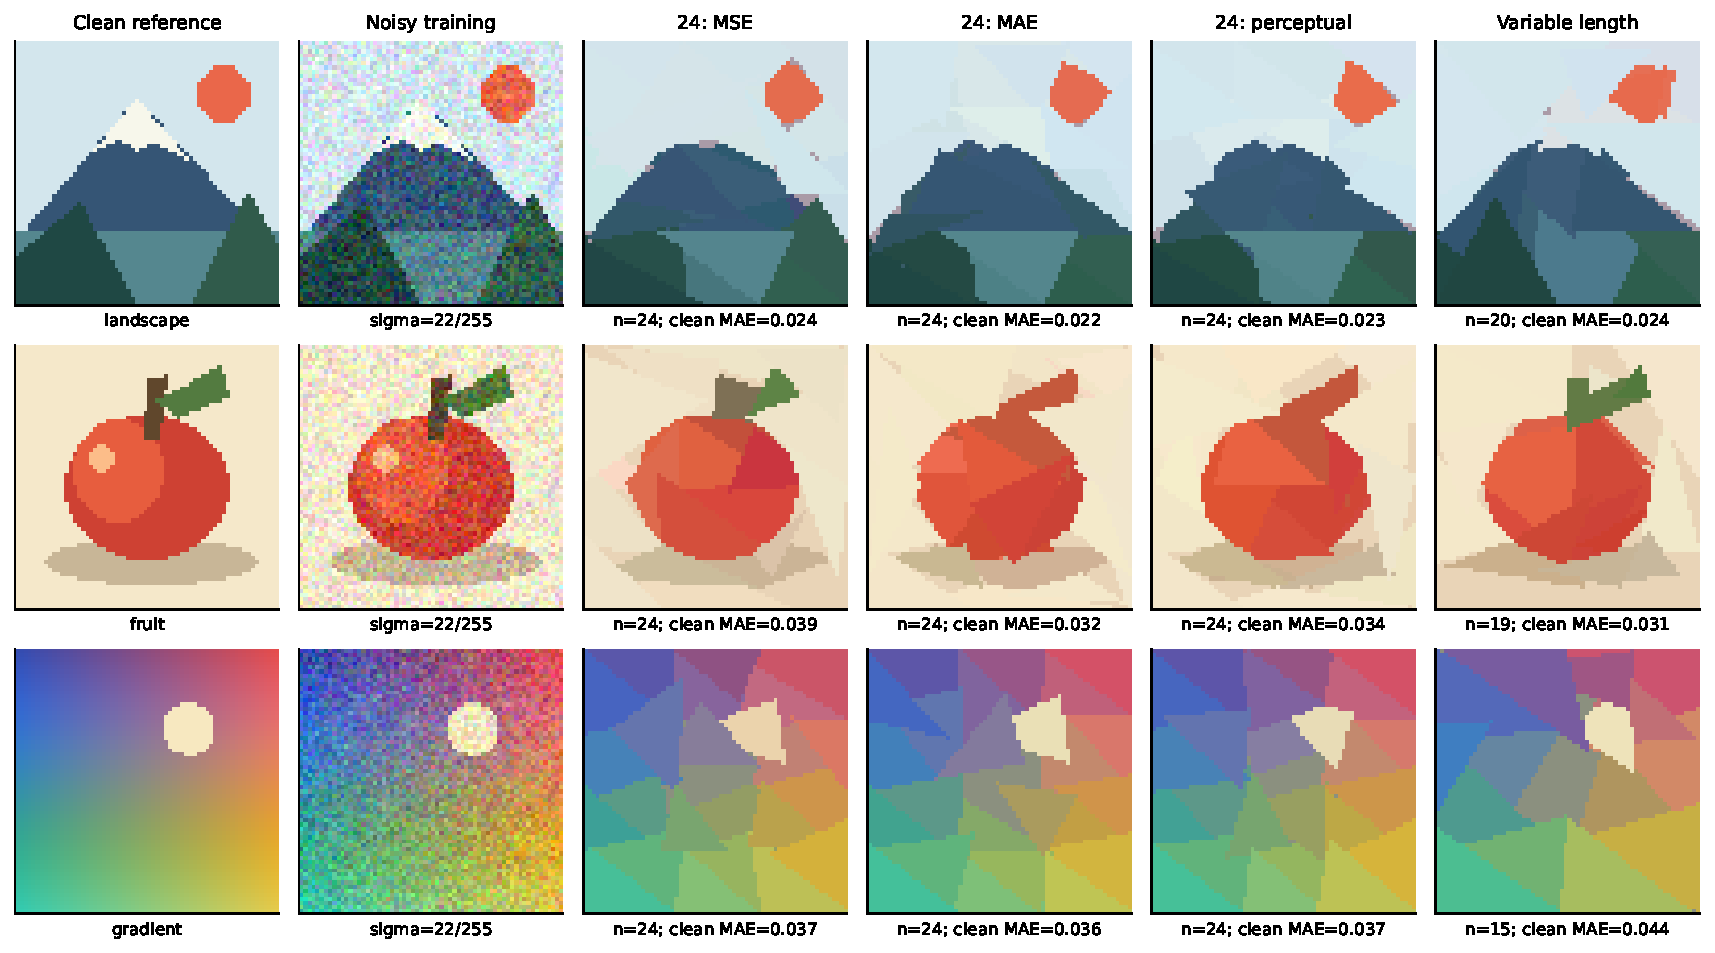
\includegraphics[width=\textwidth]{06/results/reconstructions.pdf}
\caption{第6問の入力と実測結果．各行は自作の風景・果実・勾配画像．左から原画像，ノイズを含む学習画像，24三角形のMSE・MAE・知覚代理目的，可変長表現．再現画像は事前に固定した乱数seed 0の結果であり，5回から見栄えの良いものを選んでいない．表示するclean MAEは最適化時に使っていない原画像に対する誤差である．}
\label{fig:q06_montage}
\end{figure*}

\begin{figure*}[t]
\centering
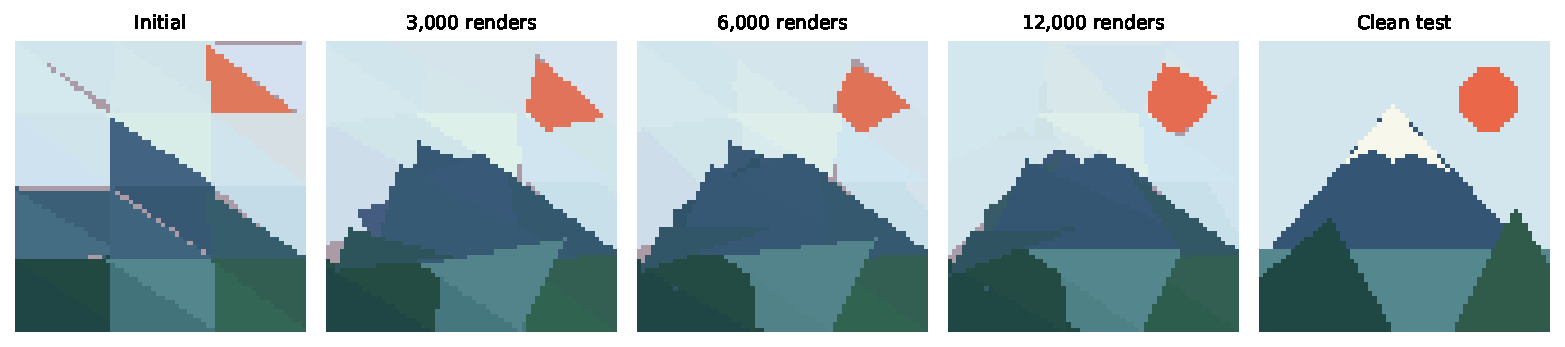
\includegraphics[width=\textwidth]{06/results/progression.pdf}
\caption{ノイズ風景・24三角形・MAE・seed 0の進化過程．初期の格子状の面が，3,000，6,000，12,000描画とともに主要境界を説明する形へ変化する．右端は探索に使っていないノイズなし参照．}
\label{fig:q06_progression}
\end{figure*}

\subsection{遺伝子型と探索手続き}
個体は順序付きリスト
\begin{equation}
 G=(t_1,\ldots,t_n),\qquad
 t_i=(x_1,y_1,x_2,y_2,x_3,y_3,r,g,b)
\end{equation}
とした．三角形は不透明であり，後に描くものが前のものを覆う．座標とRGB値を連続変数として持ち，評価時には座標を整数画素に丸める．背景は学習画像の各色成分の中央値に固定した．これは半透明色の重ね合わせによる描画とは異なり，面と輪郭の構成を明瞭に比較するための設計である．

初期集団は格子を三角分割した配置に小さい乱数摂動を与え，領域内の学習画素の平均値（MSE）または中央値（その他）で初期色を決めた．さらに突然変異の一部で同じ色推定を行う．したがって，画像の情報を初期化と提案に利用するハイブリッドGAである．目的関数の比較は，対応する平均値／中央値の色推定も組み合わせた設定間の比較であり，損失関数だけの効果を分離する実験ではない．この工夫は探索開始時から粗い色面を確保するが，学習画像へのアクセスを追加で行うため，純粋な無情報探索との優劣を主張するものではない．

基本の集団サイズは12とし，3個体のトーナメント選択，確率0.15の一点交叉，突然変異を使う．交叉は三角形リストの前半と後半を交換する．突然変異では頂点の移動，三角形の平行移動，色変更，描画順の交換を行う．新しい子1個体を評価し，集団の最悪個体より良く，かつ同じ目的値の重複でない場合に置換する$(\mu+1)$型の定常状態GAである．最良値は悪化しないが，大域最適性は保証しない．

可変長版は12三角形で初期化し，長さを2--48の範囲とした．挿入では残差が大きい場所を確率的に選んで新しい三角形を追加し，削除では1個の三角形を除く．通常の挿入分岐は8\%，削除分岐は7\%であり，長さの上下限では許された分岐のみを使う．新しい三角形の追加が必ず採択されるわけではなく，誤差改善が複雑さの費用に見合う必要がある．

\subsection{適合度と「美しさ」の定義}
RGB値を$[0,1]$に正規化し，基本目的としてMSEとMAEを比較した．さらに，色面の誤差と輪郭の誤差を組み合わせる次の代理目的を設計した．
\begin{align}
 L_{\rm p}&=\frac{\sum_{p}w_p\,d_p}{\sum_p w_p}
              +0.35\,D_{\rm edge},\\
 d_p&=\frac{1}{3}\sum_c |I_{p,c}-T_{p,c}|,\\
 w_p&=1+3\left(\overline{|\Delta_xT_p|}
                         +\overline{|\Delta_yT_p|}\right).
\end{align}
ここで$I$は描画画像，$T$は学習画像であり，$\Delta$は隣接画素の前進差分，横線はRGB平均を表す．$D_{\rm edge}$は$x,y$各方向について計算したRGB差分のMAEの平均である．画像端で存在しない差分は画素重みへの寄与を0とした．

可変長版では$L_{\rm p}+\lambda n$を最小化する．標準値は$\lambda=0.0007$とし，風景のノイズなし条件では$0$と$0.0015$も比較した．本実験での「美しさ」は，少ない面で主要な色と境界を説明するという操作的定義である．人間の主観評価を実施していないため，この目的値の低下をそのまま人間にとって美しいことの証明とはしない．

\subsection{比較条件と学習・テストの区別}
主要実験は，3画像$\times$学習画像の2条件（原画像／ノイズ画像）$\times$6設定$\times$5 seedの180試行である．6設定はMAEで8・24・48三角形，24三角形のMSE，24三角形の知覚代理目的，知覚代理目的の可変長版とした．ノイズは0--255スケールで標準偏差22の独立な正規乱数とし，範囲外をクリップした．全探索でseed 0--4を使い，学習ノイズはseed 20261117に固定した．

さらに，ノイズなし風景で集団サイズ4・36，画像に基づく色の再推定を無効化した変異，可変長の罰則2条件を各5回比較した．合計205試行，1試行12,000候補，総計2,460,000回の描画評価である．初期集団の評価もこの回数に含めた．三角形数によって1回の描画の費用は異なるため，描画数を揃えた比較に加え，実時間もJSONに記録した．

評価を終えた遺伝子を固定し，(i)ノイズなし原画像，(ii)別seed 918211のノイズ画像，(iii)太陽位置などを少し変えた類似画像，(iv)別種類の画像に対してMAE・MSE・PSNR・輪郭誤差を計算した．ノイズ学習条件では(i)の原画像を探索関数に渡しておらず，ノイズ除去の評価に使える．原画像で学習する条件では(i)が学習対象そのものなので，clean MAEは学習時の再構成誤差である．(ii)--(iv)は両学習条件とも探索に使わない．ただし，本方式は画像1枚ごとの最適化であり，画像一般を入力から変換する学習済みモデルではない．類似画像テストは固定した表現の変化への感度を調べるもので，別画像にも自動で適応できるという意味の汎化実験とは区別する．

\begin{figure}[t]
\centering
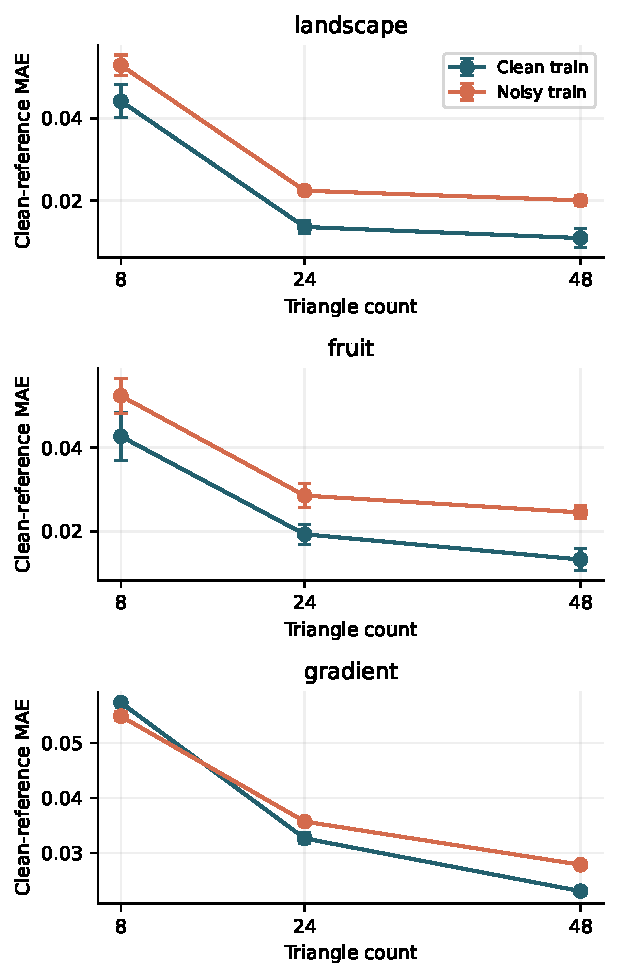
\includegraphics[width=\linewidth]{06/results/complexity.pdf}
\caption{三角形数とノイズなし参照へのMAE．原画像で学習した曲線は再構成誤差，ノイズ画像で学習した曲線は未使用の原画像への誤差である．点は5 seedの平均，誤差棒は標本標準偏差．同じ12,000描画でも，個体の次元と1描画あたりの費用は異なる．}
\label{fig:q06_complexity}
\end{figure}

\begin{table}[t]
\centering
\caption{ノイズ画像で最適化した結果の5 seed平均．評価先はノイズなし原画像．全条件の標準偏差と他の指標は公開CSVに収録した．}
\label{tab:q06_result}
\small
\begin{tabular}{llrrr}
\toprule
画像 & 適合度 & $n$ & clean MAE & edge MAE \\
\midrule
風景 & MSE & 24.0 & 0.028 & 0.015 \\
風景 & MAE & 24.0 & 0.022 & 0.016 \\
風景 & 知覚代理 & 24.0 & 0.024 & 0.016 \\
風景 & 可変長 & 18.8 & 0.024 & 0.015 \\
\midrule
果実 & MSE & 24.0 & 0.037 & 0.016 \\
果実 & MAE & 24.0 & 0.029 & 0.018 \\
果実 & 知覚代理 & 24.0 & 0.031 & 0.016 \\
果実 & 可変長 & 16.2 & 0.033 & 0.016 \\
\midrule
勾配 & MSE & 24.0 & 0.037 & 0.014 \\
勾配 & MAE & 24.0 & 0.036 & 0.014 \\
勾配 & 知覚代理 & 24.0 & 0.036 & 0.014 \\
勾配 & 可変長 & 15.6 & 0.043 & 0.013 \\
\bottomrule
\end{tabular}

\end{table}

\subsection{実行結果}
図\ref{fig:q06_montage}のように，風景では山・雪・太陽・水面の主要構造，果実では丸い輪郭と葉，勾配では色の方向性が獲得された．同じ三角形でも，対象が角張った構造か曲線かによって必要な面の使い方が異なる．三角形数を増やすと表現の自由度が増える一方，限られた候補数で調整すべき頂点と色も増える．

ノイズなし風景のMAEは，8三角形で平均0.0442，24三角形で0.0136，48三角形で0.0109であった．24から48への改善幅は8から24への改善幅より小さい．また，可変長版は平均22.4三角形でMAE 0.0114となり，固定24のMAE版より少ない面で低い誤差を得た．ただし，目的関数と挿入操作も同時に異なるため，この差を長さ可変化だけの因果効果とは解釈しない．

可変長の罰則を$0,\,0.0007,\,0.0015$としたとき，ノイズなし風景の平均三角形数は$43.4,\,22.4,\,16.2$，clean MAEは$0.0068,\,0.0114,\,0.0190$となった．少ない三角形で描くには，ある程度の忠実さを明示的に譲る必要がある．また，集団サイズ4・12・36の固定24三角形MAE版は，それぞれ$0.0109,\,0.0136,\,0.0168$であった．本条件では小集団の方が良かったが，これは同じ評価回数での結果であり，多様性を増せば必ず改善するとは限らないことを示す．画像に基づく変異時の色再推定を無効にした版は$0.0132$で，標準版$0.0136$に対する明瞭な劣化は観察されなかった．提案した工夫をすべて有効だったと解釈せず，改善が必要な要素として扱う．

ノイズを含む風景では，24三角形MAE版のclean MAEは0.0224，MSE版は0.0282，知覚代理版は0.0237であった．一方，輪郭誤差はそれぞれ0.0162，0.0154，0.0162であり，知覚代理版が常に最良にはならなかった．これらは，MAEと中央値色，MSEと平均色，知覚代理目的と中央値色を組み合わせた各設定が到達した妥協点であり，色推定も異なるため損失関数だけの因果効果には分解できない．本実験から知覚代理設定の美的優越性は確認できない．ノイズ自体も勾配を増やすため，学習画像から作った輪郭重みにはノイズを強調する危険もある．

同じ24三角形MAE版の固定遺伝子を別の参照に評価すると，学習ノイズ画像へのMAEは$0.0749\pm0.0007$，独立ノイズ画像では$0.0763\pm0.0007$，類似風景では$0.0298\pm0.0011$，別画像の果実では$0.3061\pm0.0011$となった（平均$\pm$標本標準偏差）．入力ノイズ画像自体のclean MAE 0.0655に対し，再構成では$0.0224\pm0.0010$へ低下した．細かな学習ノイズの複製より大きな構造の近似が進んだことが分かる．一方，太陽の位置などを変えると誤差が増え，別対象への置換では大きく崩れる．これは1枚の表現を固定したことによる感度であり，画像認識器の汎化性能とは異なる．

\begin{figure}[t]
\centering
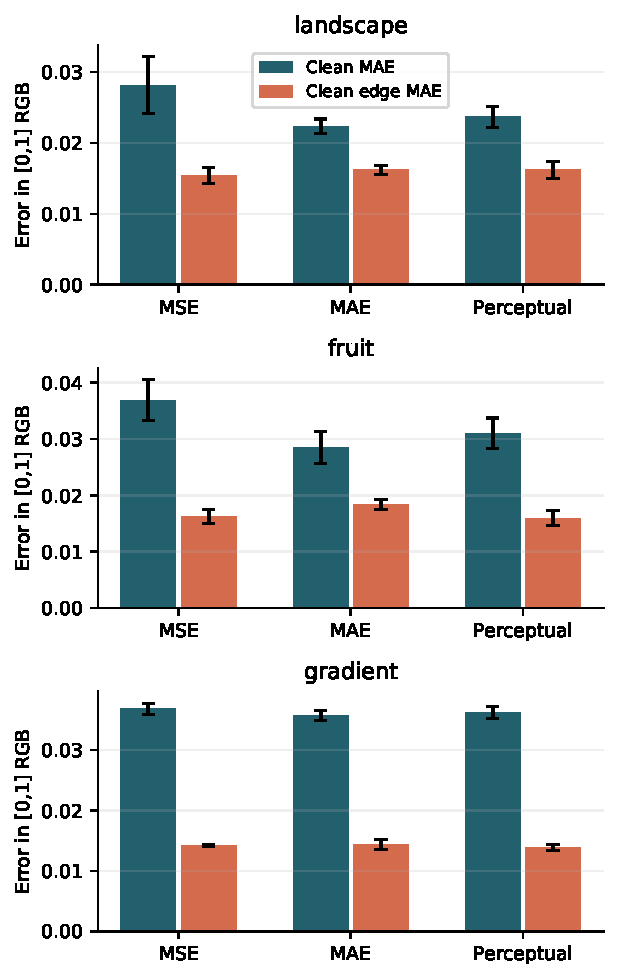
\includegraphics[width=\linewidth]{06/results/objectives.pdf}
\caption{ノイズ画像に学習した24三角形のclean MAEと輪郭MAE．目的関数と対応する色推定（MSEは平均値，その他は中央値）を組み合わせた設定の比較であり，損失関数だけの比較ではない．平均と標本標準偏差を示す．}
\label{fig:q06_objectives}
\end{figure}

\begin{figure}[t]
\centering
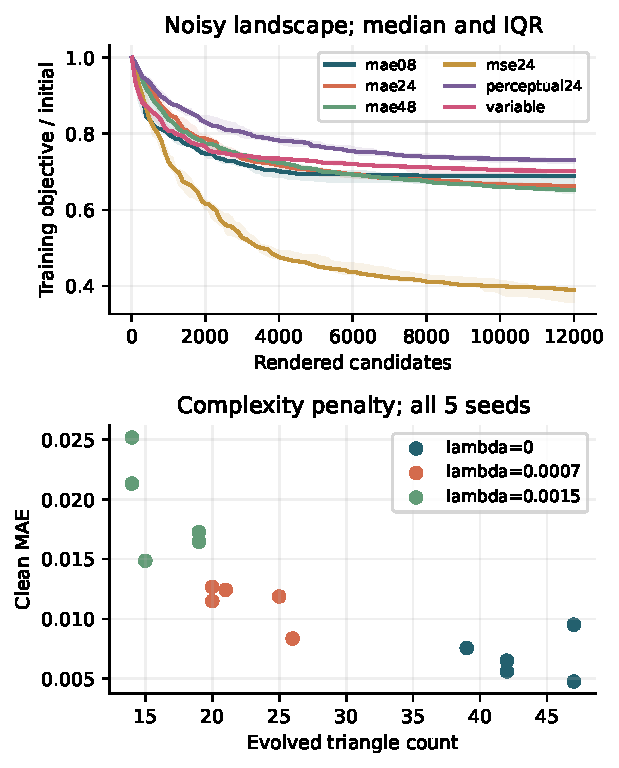
\includegraphics[width=\linewidth]{06/results/evolution_pareto.pdf}
\caption{上：ノイズを含む風景の探索推移（中央値と四分位範囲）．縦軸は各条件自身の初期目的値で割った比であり，異なる目的関数の絶対値を同一尺度として比較していない．下：ノイズなし風景の可変長版で，複雑さ罰則を変えた各seedの三角形数とMAE．}
\label{fig:q06_pareto}
\end{figure}

\subsection{考察と改善案}
三角形の枚数は一種の正則化として働く．少ない面しか使えないため，各画素に独立なノイズをそのまま記憶しにくい．他方，極端に少ない面では葉や雪の境界も消えてしまう．$\lambda n$の費用は，この複雑さと忠実さの選択を明示的に表している．本実験では少数の独立な探索seedしか扱っていないため，小さな平均差を統計的な一般則と断定しない．

適用範囲も限定される．ここで扱ったのは小さい合成画像3種類であり，自然写真，大きい解像度，半透明表現，多人数による主観評価は未検証である．特に滑らかな勾配を不透明な一定色の三角形で表すと，少数の面では色の段差が残る．対象の性質に合わせて表現自体を変えることも，探索方法を改良することと同程度に重要である．

知覚項については，人間が重要だと感じる境界と，単に数値的に強い局所差分を区別することが次の課題である．例えばノイズを抑えた複数解像度の輪郭，知覚色空間での色差，主対象に重みを付けるマスクを導入できる．ただし，目的項が増えるほど探索が難しくなるため，候補数一定の場合と計算時間一定の場合の両方で比較する必要がある．

人間の好みを直接扱うにはIECも有望である．例えば，誤差と三角形数のパレート前線上の候補を少数だけ提示し，「どちらが好ましいか」の対比較から選好モデルを作れば，単一のMAE値より感覚を反映できる可能性がある．その際は，評価者数，提示順のランダム化，疲労，個人差を記録すべきである．今回は人間の評価を実施していないため，IECによる改善や美的優越性は主張しない．

再現性のため，元画像生成コード，乱数seed，最終遺伝子，全試行の目的値と所要時間，収束履歴を保存した．表と図は同じJSONから再生成する．また，公開JSONからPNGとSVGを出力できる．SVGは連続座標を保つため，整数画素に丸めた評価用画像とは境界がわずかに異なる点をREADMEに明記した．

\repolink{06}
\clearpage
\section*{講義へのコメント}
異なる問題でも、表現方法と評価指標によって探索結果の意味が変わることを確かめられた。
探索の展開数やGAの世代数に加え、適合度評価回数と計算時間を併記する比較が特に有益であった。
授業で使用するベンチマークに機械可読な配列・正解検証器が添付されると、入力の転記ミスを避け、発展的な実験に時間を使えると考える。
\begin{thebibliography}{99}
\bibitem{nobel} Nobel Foundation. The Nobel Prize in Chemistry 2024, press release (2024). \url{https://www.nobelprize.org/prizes/chemistry/2024/press-release/}
\bibitem{foldit} Foldit. Official help / Rosetta documentation. \url{https://dev.fold.it/help}\quad\url{https://docs.rosettacommons.org/docs/latest/FoldIt}
\bibitem{cooper} Cooper, S. et al. Predicting protein structures with a multiplayer online game. Nature 466, 756--760 (2010). DOI: \url{https://doi.org/10.1038/nature09304}
\bibitem{kosinski} Kosinski, M. Evaluating large language models in theory of mind tasks. PNAS 121(45), e2405460121 (2024). \url{https://doi.org/10.1073/pnas.2405460121}
\bibitem{strachan} Strachan, J. W. A. et al. Testing theory of mind in large language models and humans. Nature Human Behaviour 8, 1285--1295 (2024). \url{https://doi.org/10.1038/s41562-024-01882-z}
\bibitem{tomreview} Chen, R., Jiang, W., Qin, C., Tan, C. Theory of Mind in Large Language Models: Assessment and Enhancement. ACL (2025). \url{https://arxiv.org/abs/2505.00026}
\bibitem{xenobot} Kriegman, S., Blackiston, D., Levin, M., Bongard, J. Kinematic self-replication in reconfigurable organisms. PNAS 118(49), e2112672118 (2021). \url{https://doi.org/10.1073/pnas.2112672118}
\bibitem{wyss} Wyss Institute. Team builds first living robots that can reproduce (2021). \url{https://wyss.harvard.edu/news/team-builds-first-living-robots-that-can-reproduce/}
\bibitem{hart1968} Hart, P. E., Nilsson, N. J., Raphael, B. A Formal Basis for the Heuristic Determination of Minimum Cost Paths. IEEE Transactions on Systems Science and Cybernetics 4(2), 100--107 (1968). \url{https://doi.org/10.1109/TSSC.1968.300136}
\end{thebibliography}

\end{document}
